% This sample file is dedicated to the public domain.
\documentclass[12pt]{myucthesis}

%\nofiles
% The above command prevents latex from writing its auxiliary
% files. This is useful if you want to manually tweak them before you
% generate your final PDF.


% Page layout. The fancyhdr package may complain about the need for a
% larger headheight, depending on how long chapter titles are; if left
% unspecified in the geometry setup, it defaults to 12pt. The
% "showframe" option causes the geometry package (version >= 5.0) to
% show a frame around the margins on every page, which is great for
% checking that you don't overflow anywhere.

%\usepackage[letterpaper,includehead,margin=1in,headheight=15pt,showframe]{geometry}
\usepackage[letterpaper,includehead,margin=1in,headheight=15pt]{geometry}
\usepackage{fancyhdr}
\pagestyle{fancyplain}
\lhead[\fancyplain{\thepage}{\thepage}]{\fancyplain{}{\scshape\rightmark}}
\rhead[\fancyplain{}{\scshape\leftmark}]{\fancyplain{\thepage}{\thepage}}
\chead{}
\cfoot{}
\lfoot{}
\rfoot{}


% Bibliography stuff:

\newcommand{\newblock}{\par} % need this for some natbib internal bug
\usepackage{natbib}
\citestyle{aa}
\bibliographystyle{yahapj}
\setlength{\bibsep}{0ex} % single-space entries
\def\bibpreamble{\addcontentsline{toc}{chapter}{Bibliography}} % get a good TOC entry


% Other setup:

\usepackage[T1]{fontenc} % see http://tinyurl.com/67zdxwf
\usepackage[colorlinks,urlcolor=blue,citecolor=blue,linkcolor=blue,pdfusetitle]{hyperref}
\usepackage{pdflscape} % allows landscape-oriented figures with PDF page rotation
\usepackage{aasmacros,amsmath,amssymb,graphicx}
\usepackage{mydeluxetable} % deluxetable customized to play well with ucthesis


% ralf imports 
% Smart references
\usepackage[capitalize]{cleveref}
\usepackage{multirow}
%\usepackage[table]{colortbl}
\usepackage[a-2b]{pdfx}
\crefformat{section}{#2\S#1#3}
%\crefname{section}{\S}{\S}
\crefname{listing}{Lst.}{Lst.}


\newcommand{\system}{RALF}

% Conditionals (for draft mode)
\usepackage{ifthen}
% Special fractions
\usepackage{nicefrac}

% listings 
\usepackage{listings}
%\usepackage{xcolor}
\lstloadlanguages{Python}

% Subfigures
\usepackage{caption}
\usepackage{subcaption}

% Algorithms
\usepackage{algorithm}
%\SetKwComment{Comment}{/* }{ */}

% Bolded paragraphs.
\newcommand{\myparagraph}[1]{\noindent{\bfseries #1.}}

% argmax 
\usepackage{amsmath}
\DeclareMathOperator*{\argmax}{arg\,max}
\DeclareMathOperator*{\argmin}{arg\,min}

% TODO Comments.
\newif\ifcomments
\commentstrue
\commentsfalse
\ifcomments
\usepackage[textsize=small,color=lightgray]{todonotes}
\else
\usepackage[disable]{todonotes}
\fi

% TODO: add yourself
\newcommand{\sarah}[1]{\todo[color=cyan!40]{\textbf{Sarah}: #1}\ignorespaces}
\newcommand{\joey}[1]{\todo[color=green!50]{\textbf{Joey}: #1}\ignorespaces}
\newcommand{\important}[1]{\todo[color=red!50]{\textbf{Important}: #1}\ignorespaces}
\newcommand{\amit}[1]{\todo[color=yellow!50]{\textbf{Amit}: #1}\ignorespaces}
\newcommand{\natacha}[1]{\todo[color=orange!50]{\textbf{Natacha}: #1}\ignorespaces}
\newcommand{\kevin}[1]{\todo[color={magenta!40}]{\textbf{Kevin}: #1}\ignorespaces}
\newcommand{\simon}[1]{\todo[color={gray!40}]{\textbf{Simon}: #1}\ignorespaces}
\newcommand{\jmh}[1]{\todo[color={gray!40}]{\textbf{JMH}: #1}\ignorespaces}

% Increase page size if comments.         
\ifcomments                                                                     
% Increase page size without affecting formatting
\paperwidth=\dimexpr \paperwidth + 8cm\relax
\oddsidemargin=\dimexpr\oddsidemargin + 4cm\relax
\evensidemargin=\dimexpr\evensidemargin + 4cm\relax
\marginparwidth=\dimexpr \marginparwidth + 3cm\relax            
\fi

%\RequirePackage[loading]{tracefnt}
%\usepackage[weather]{ifsym}

%% These commands are for a PROCEEDINGS abstract or paper.
%\acmConference[SIGMOD '23]{}{Jyune 03--05, 2018}{Woodstock, NY}
%
%  Uncomment \acmBooktitle if th title of the proceedings is different
%  from ``Proceedings of ...''!
%
%\acmBooktitle{Woodstock '18: ACM Symposium on Neural Gaze Detection,
%  June 03--05, 2018, Woodstock, NY} 
%\acmPrice{15.00}
%\acmISBN{978-1-4503-XXXX-X/18/06}


%%
%% Submission ID.
%% Use this when submitting an article to a sponsored event. You'll
%% receive a unique submission ID from the organizers
%% of the event, and this ID should be used as the parameter to this command.
%\acmSubmissionID{32}




\begin{document}
\ssp % single spacing
\hypersetup{pageanchor=false}
\title{My Amazing Thesis}
\author{Sarah Wooders} % must match BearFacts!
\degreesemester{Fall}
\degreeyear{2012}
\degree{Doctor of Philosophy}
\numberofmembers{3}
\chair{Professor Natacha Crooks}
\othermembers{
Professor Ion Stoica \\
Professor Joseph E. Gonzalez \\
Professor Vincent Liu 
}
\field{EECS}
\campus{Berkeley}

\maketitle
\copyrightpage

\begin{abstract}
My work is awesome. Give me a Ph.D.
\end{abstract}

\hypersetup{pageanchor=true}
\begin{frontmatter}

\begin{dedication}
\null\vfil
{\large
\begin{center}
I dedicate this dissertation to graduate students everywhere.
\end{center}}
\null\vfil
\end{dedication}

\tableofcontents
\listoffigures % optional
\listoftables % optional

% If using code.sty, can also add:
%% \listofcodes
%% \addcontentsline{toc}{chapter}{List of Code Examples}

\begin{acknowledgements}
Too bad nobody helped me.

% Feel free to modify or remove this acknowledgment:
This dissertation was typeset using the
\href{https://github.com/pkgw/ucastrothesis}{\textsf{ucastrothesis}}
\LaTeX\ template.

\end{acknowledgements}
\end{frontmatter}

% This sample file is dedicated to the public domain.
\chapter{Introduction}
\label{c.intro}

Abstract.

\section{Introduction}

This is some stuff about science. I feel a strange compulsion to cite
\citet{williams12}.

\section{Feelings on My Thesis}


\section*{Acknowledgments}

Too bad nobody helped me with the introduction either.


% ralf 

% VLDB template version of 2020-08-03 enhances the ACM template, version 1.7.0:
% https://www.acm.org/publications/proceedings-template
% The ACM Latex guide provides further information about the ACM template


%\documentclass[sigconf, nonacm, authordraft]{acmart}
%\documentclass[sigconf, nonacm, pdfa]{acmart}
%% The following content must be adapted for the final version
% paper-specific
\newcommand\vldbdoi{10.14778/3632093.3632116}
\newcommand\vldbpages{563-576}
% issue-specific
\newcommand\vldbvolume{17}
\newcommand\vldbissue{3}
\newcommand\vldbyear{2023}
% should be fine as it is
\newcommand\vldbauthors{\authors}
\newcommand\vldbtitle{\shorttitle} 
% leave empty if no availability url should be set
\newcommand\vldbavailabilityurl{https://github.com/feature-store/ralf}
% whether page numbers should be ™shown or not, use 'plain' for review versions, 'empty' for camera ready
\newcommand\vldbpagestyle{empty} 



%\begin{document}
%\title{\system{}: Accuracy-Aware Scheduling for Feature Store Maintenance}
%\title{\system{}: Accuracy-Aware Maintenance for Embedding \& Feature Stores}
\title{\system{}: Accuracy-Aware Scheduling for Feature Store Maintenance}
%
%% The "author" command and its associated commands are used to define the authors and their affiliations.
%\author{Sarah Wooders}
%\affiliation{%
%  \institution{UC Berkeley}
%}
%\email{wooders@berkeley.edu}
%
%\author{Xiangxi Mo}
%\affiliation{%
%  \institution{UC Berkeley}
%}
%\email{xmo@berkeley.edu}
%
%
%\author{Amit Narang}
%\affiliation{%
%  \institution{UC Berkeley}
%}
%\email{narang@berkeley.edu}
%
%\author{Kevin Lin}
%\affiliation{%
%  \institution{UC Berkeley}
%}
%\email{k-lin@berkeley.edu}
%
%\author{Ion Stoica}
%\affiliation{%
%  \institution{UC Berkeley}
%}
%\email{istoica@berkeley.edu}
%
%\author{Joseph M. Hellerstein}
%\affiliation{%
%  \institution{UC Berkeley}
%}
%\email{hellerstein@berkeley.edu }
%
%\author{Natacha Crooks}
%\affiliation{%
%  \institution{UC Berkeley}
%}
%\email{ncrooks@berkeley.edu}
%
%\author{Joseph E. Gonzalez}
%\affiliation{%
%  \institution{UC Berkeley}
%}
%\email{jegonzal@berkeley.edu }
% \author{Lars Th{\o}rv{\"a}ld}
% \orcid{0000-0002-1825-0097}
% \affiliation{%
%   \institution{The Th{\o}rv{\"a}ld Group}
%   \streetaddress{1 Th{\o}rv{\"a}ld Circle}
%   \city{Hekla}
%   \country{Iceland}
% }
% \email{larst@affiliation.org}

% \author{Valerie B\'eranger}
% \orcid{0000-0001-5109-3700}
% \affiliation{%
%   \institution{Inria Paris-Rocquencourt}
%   \city{Rocquencourt}
%   \country{France}
% }
% \email{vb@rocquencourt.com}

% \author{J\"org von \"Arbach}
% \affiliation{%
%   \institution{University of T\"ubingen}
%   \city{T\"ubingen}
%   \country{Germany}
% }
% \email{jaerbach@uni-tuebingen.edu}
% \email{myprivate@email.com}
% \email{second@affiliation.mail}

% \author{Wang Xiu Ying}
% \author{Zhe Zuo}
% \affiliation{%
%   \institution{East China Normal University}
%   \city{Shanghai}
%   \country{China}
% }
% \email{firstname.lastname@ecnu.edu.cn}

% \author{Donald Fauntleroy Duck}
% \affiliation{%
%   \institution{Scientific Writing Academy}
%   \city{Duckburg}
%   \country{Calisota}
% }
% \affiliation{%
%   \institution{Donald's Second Affiliation}
%   \city{City}
%   \country{country}
% }
% \email{donald@swa.edu}

%%
%% The abstract is a short summary of the work to be presented in the
%% article.
\begin{abstract}
Feature stores (also sometimes referred to as embedding stores) are becoming ubiquitous in model serving systems: downstream applications query these stores for auxiliary inputs at inference-time. Stored features are derived by \textit{featurizing} rapidly changing base data sources. Featurization can be costly prohibitively expensive to trigger on every data update, particularly for features that are vector embeddings computed by a model. Yet, existing systems naively apply a one-size-fits-all policy as to when/how to update these features, and do not consider query access patterns or impacts on prediction accuracy. 
This paper introduces \system{}, which orchestrates feature updates by leveraging \textit{downstream error feedback} to minimize \textit{feature store regret}, a metric for how much featurization degrades downstream accuracy. We evaluate with representative feature store workloads, anomaly detection and recommendation, using real-world datasets. We run system experiments with a 275,077 key anomaly detection workload on 800 cores to show up to a 32.7\% reduction in prediction error or up to $1.6\times$ compute cost reduction with accuracy-aware scheduling. 
%\textcolor{red}{For resource constrained settings, we demonstrate up to 30\% improvements in downstream prediction accuracy for an information retrieval task, and loss reductions of up to 23\% for estimating time-series anomalies.}
\end{abstract}



\maketitle

%%% do not modify the following VLDB block %%
%%% VLDB block start %%%
%\pagestyle{\vldbpagestyle}
%\begingroup\small\noindent\raggedright\textbf{PVLDB Reference Format:}\\
%\vldbauthors. \vldbtitle. PVLDB, \vldbvolume(\vldbissue): \vldbpages, \vldbyear.\\
%\href{https://doi.org/\vldbdoi}{doi:\vldbdoi}
%\endgroup
%\begingroup
%\renewcommand\thefootnote{}\footnote{\noindent
%This work is licensed under the Creative Commons BY-NC-ND 4.0 International License. Visit \url{https://creativecommons.org/licenses/by-nc-nd/4.0/} to view a copy of this license. For any use beyond those covered by this license, obtain permission by emailing \href{mailto:info@vldb.org}{info@vldb.org}. Copyright is held by the owner/author(s). Publication rights licensed to the VLDB Endowment. \\
%\raggedright Proceedings of the VLDB Endowment, Vol. \vldbvolume, No. \vldbissue\ %
%ISSN 2150-8097. \\
%\href{https://doi.org/\vldbdoi}{doi:\vldbdoi} \\
%}\addtocounter{footnote}{-1}\endgroup
%%% VLDB block end %%%

%%% do not modify the following VLDB block %%
%%% VLDB block start %%%
%\ifdefempty{\vldbavailabilityurl}{}{
%\vspace{.3cm}
%\begingroup\small\noindent\raggedright\textbf{PVLDB Artifact Availability:}\\
%The source code, data, and/or other artifacts have been made available at \url{\vldbavailabilityurl}.
%\endgroup
%}



%%%%%%%%%%%%%%%%%%%%%%%%%%%%%%%%%%%%%%%%%%%%%%%%%%%%%%%%%%%%%%%%%%%%%%%%%%%%
% INTRODUCTION
%%%%%%%%%%%%%%%%%%%%%%%%%%%%%%%%%%%%%%%%%%%%%%%%%%%%%%%%%%%%%%%%%%%%%%%%%%%%
\section{Introduction}
\begin{figure}[t]
\centering
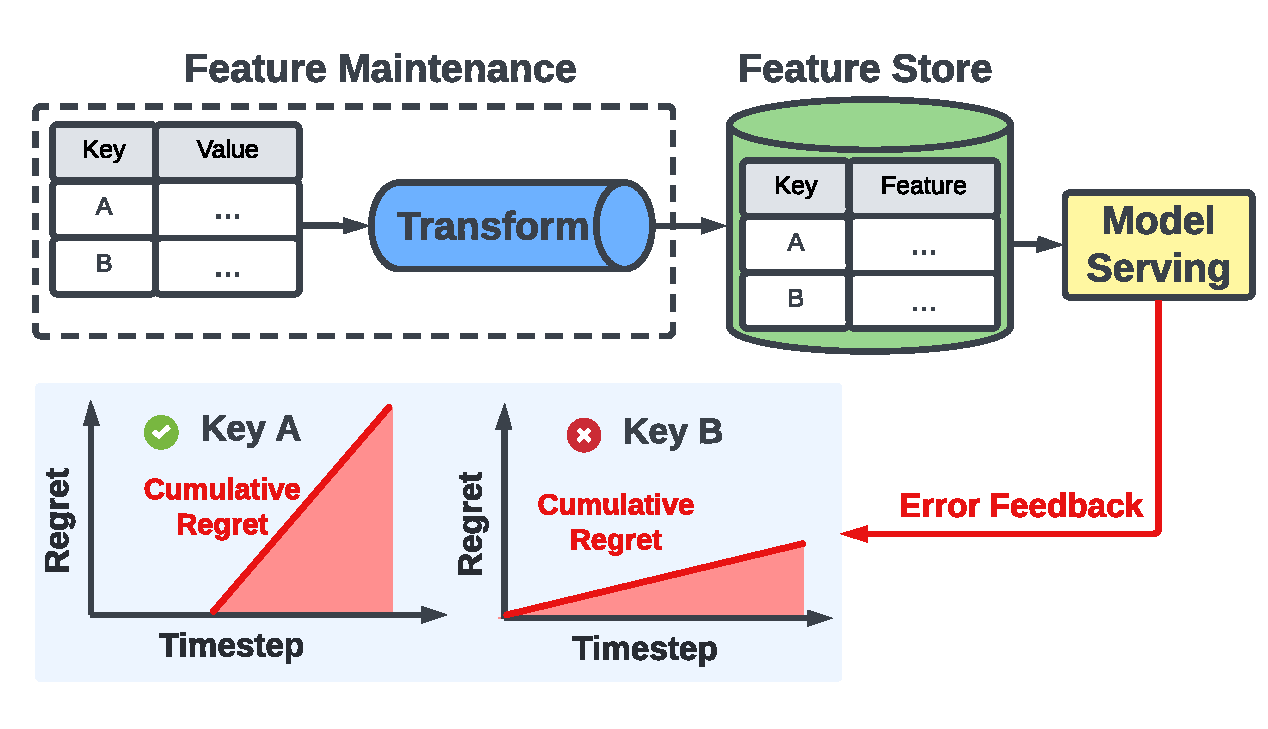
\includegraphics[width=8.5cm]{ralf/figures/overview.pdf}
%\setlength{\abovecaptionskip}{-0pt}
%\setlength{\belowcaptionskip}{-20pt}
\caption{Feature stores serve materialized feature values to downstream models. 
%Computationally expensive feature maintenance pipelines are used to update feature values when the underlying data changes in a best effort fashion.
%However, stale feature values can significantly degrade prediction quality in a manner that depends on the model and feature access pattern. 
\system{} leverage downstream model feedback to prioritize expensive feature updates (\cref{ss:scheduling-policy}).}


\label{f:overview}
\end{figure}

\label{s:introduction}
%This paper describes Ralf, a feature store that explicitly leverages downstream feedback to intelligently schedule feature recomputation.

% \natacha{I find a first sentence that describes the paper, before going into the real intro, to be useful.
% This paper describes Ralf, a feature store that explicitly leverages downstream feedback to intelligently
% schedule feature recomputation}
Most real-world applications of machine learning rely heavily on pre-computed \emph{features} to improve model accuracy and reduce prediction latency.
Features are raw and derived data that are passed as input to machine learning models to capture the context around a prediction.
For example, fraud detection and content recommendation models rely on features describing merchants, users, and content to make accurate predictions. More recently, large language models increasingly depend on features of relevant context (eg. embeddings of past conversational history) to provide more grounded and personalized responses \cite{lee2019latent, guu2020retrieval, packer2023memgpt, lewis2020retrieval}.

%Features include both raw data (e.g., the price of a product) as well as derived data (e.g., a embedding representation of a product) that may require significant computation. 


% \joey{adding a running example really early.}
Consider for example an online news recommendation service that predicts the probability that a specific user will click on specific article.
Standard models for this task \cite{koren2009matrix,DLRM19}
% \joey{cite DLRM and matrix factorization work.}
rely on sophisticated features (such as model based embedding) that summarize the 
user's click history, the text in the article, and the click histories of other users that have clicked on that article.
These features are critical to making good predictions, but are expensive to compute and sensitive to the continuously changing news cycle. 
% \natacha{Not for MLSys, but if we submit elsewhere, it's a little confusing to think of features as part
% of something that is outside of the model, when it feels like it should already been captured in the mode (like the click history, isn't that what you're training on already?) Not for MLSys, but for a less ML heavy conference, might be useful to clarify }
% \joey{In a future cut of this paper we might pull more from section 2 into the introduction to address Natacha's concern}





% In these settings, predictions must be made in 10s of milliseconds but often depend on complex analysis of historical data (e.g., user purchase or click history).
% % in real time. Real-time serving systems are often subjected to tight latency constraints (<100ms), limiting the amount of data retrieval and computation that can be done when a prediction is requested \cite{crankshaw2020inferline}.  
% As a result, prediction serving system often rely on pre-computed \emph{features} (e.g., user purchasing patterns) in addition to query specific inputs (e.g., items in the cart) to provide low-latency, accurate predictions. 

%\joey{This paragraph is good but maybe redundant with the first?  There might be enough example in the above paragraph to drop this one. Actually, the one thing that maybe isn't clear at this point is that features are keyed by the query.}
% Features are derived from computations such as embeddings or large aggregations and often specific to a model query.
% For example, news recommendation models 
% % may use both the current shopping cart items (provided by the prediction request) and a 
% rely on features vectors representing both the historical preferences of each user as well as properties of each article. 
% These feature vectors are typically computed by running historical data through featurization transformations 
% ranging from simple aggregates to complex embedding models.
% When ranking articles for a given user, the features associated with that user and any candidate articles, along with session information are then passed to the news recommendation model.


% However, as users interact with the system the features of both the users and the articles change and those changes often reflect important s


%As users view content their feature

% to encode the historical interests of users and the characteristics of users that click on each article.


% as well as key properties of the hosted content.

% behavior and product ratings into a representative vector. 

Real-time model serving applications, such as online news recommendation services, require low latency predictions, and therefore rely heavily on pre-materialized \emph{feature tables} stored and maintained by a \emph{feature store} to hide the latency associated with deriving features. 
In order to provide low-latency access to important contexual information, \emph{feature tables}
At prediction time, the model serving system 
queries the pre-computed features from the
feature store by specifying a \textit{feature key} (e.g. a user ID), as shown in \cref{f:overview}. 
However, because the features are often derived from data that is constantly changing (e.g., click streams and purchase history), the pre-materialized features also need to be continuously updated with the arrival of new data.
% This process of updating features in response to changing data is the responsibility of the feature store system.
Unfortunately, updating features with every data change can be wasteful and  expensive for high-velocity data streams if the features are not read between updates or cannot be updated incrementally. Beyond computation cost, featurization via third party services also may impost hard rate limits on model-based embedding computations \cite{openai, cohere}. 

\kevin{Discuss potential issues with rate limits also here.
 
 "Beyond computational cost, featurization often uses third party services that impose hard rate limits that constrain the number of featurization updates over a time period. <Add some numbers from common embedding APIs eg. openai, cohere>:"


 https://cohere.com/pricing
 https://platform.openai.com/docs/guides/rate-limits/usage-tiers?context=tier-free

 
 }




% Unfortunately, many of the expensive featurization operations don't have incremental update strategies and so maintaining up-to-date features can be prohibitively expensive.  
% \natacha{You could be more direct here: Existing model
% prediction pipelines are faced with a binary choice
% 1) greedily recomputing features on every input 2) allowing features to become arbitrarily stale. The former is often prohibitive performance-wise while the latter significantly degrades downstream model performance, as shown in Figure 3. 
% This trade-off is not unusual in this space: weakly consistent datastores are faced with similar issues. Relaxing consistency and allowing for stale data can break correctness in ways that are difficult to quantity (cite).  In the specific context of feature stores, however, a third alternative is possible. There exists a clean, measurable metric that one can use as a guide for when and how to compute features:downstream model accuracy. Downstream model accuracy is DEFINE. Using this observation, we can reframe the problem of building a resource-efficient feature store: rather than treating featurisation as ... we can view it as an optimisation problem that seaks to maximise downstream model accuracy. }
%As a consequence, a common solution to feature maintenance is to apply a best effort approach to updating features as new data arrives, which often results in stale or approximated features. 
%While models have some degree of tolerance for stale features, we find that features which are stale or inaccurate often significantly degrade downstream model performance, as show in Figure \cref{fig:staleness}. 

As a consequence, existing feature stores are faced with a choice between (1) greedily processing new updates as they arrive, and (2) allowing features to become arbitrarily stale. 
The former is often prohibitively resource intensive while the latter significantly degrades downstream model accuracy, as shown in \cref{f:staleness}. 
This trade-off is not unusual in this space: weakly consistent data stores are faced with similar issues. In general, relaxing consistency and allowing for stale data can break correctness in ways that are difficult to quantify \cite{sivasubramanian2012amazon,cooper2008pnuts}. 
% \sarah{cite} \jmh{in general}. \natacha{PNUTS, dynamo, cops, tardis, bayou, and a gazillion more}

In the specific context of feature stores, however, ``breaking correctness'' has a measurable metric: \emph{downstream model accuracy}. This is a clean %, measurable 
metric that quantifies the prediction accuracy of a deployed model serving predictions. We can use downstream model accuracy as a guide for when and how to compute features and reframe the problem of building a resource-efficient feature store; rather than treating featurization as a task-agnostic data processing problem, we focus on maximizing downstream model accuracy.

% To address this generality, ``staleness'' in storage systems is often measured in terms of the \emph{number of updates} to a data item, rather than the application-relevant \emph{content} of the updated item.\natacha{See slack for suggested rephrasing}
% In the specific context of feature stores, however, a third alternative is possible. There exists a clean, measurable metric that one can use as a guide for when and how to compute features: downstream model accuracy. Downstream model accuracy measures the prediction accuracy of a deployed model serving predictions.  Using this observation, we can reframe the problem of building a resource-efficient feature store; rather than treating featurization as a task-agnostic data processing problem, we focus on maximizing downstream model accuracy.

We find that the appropriate feature maintenance 
policy for optimizing downstream accuracy can be key-dependent (within a single feature table) and vary across time.
%\natacha{varies across time feels a little strange; it sounds like you're changing the policy itself, rather than when you recompute. We find that deciding when to recompute a feature for optimizing downstream accuracy is both key and time dependent}
Keys that are rarely queried are unlikely to have significant impacts on overall downstream accuracy. 
%Hotspot keys are also frequent in real workloads, as we show in \cref{f:updates_vs_queries}, and do not necessarily correspond to the keys with the most new incoming data. 
Furthermore, even if keys are queried and updated at similar rates, the impact of staleness on accuracy varies dramatically by key. For example, some keys can be updated much less frequently than others without significantly impacting downstream accuracy, as show in \cref{f:update_variance}.
 Prioritizing updates across keys can enable better resource efficiency in optimizing for downstream model accuracy. 


%A stale feature that changes very little with new data or that is rarely queried by downstream tasks is less likely to affect accuracy, offering opportunities for saving on resource cost. 

%, suggesting that the scheduling feature updates should be fine-grained and adaptable. The effect of feature staleness on downstream accuracy can vary between different types of features, or even features within the same feature table.

%A fundamental trade-off with maintaining features is between feature pipeline cost and inference accuracy. Roughly speaking, updating features more frequently reduces the probability of downstream accuracy degradation, but also incurs higher compute resource costs. 



%\sarah{The VLDB paper referred to this as model staleness rather than feature staleness - maybe we can do that do and refer to prior work on data drift?}
%The degree to which feature staleness degrades downstream accuracy can vary between different types of features, or even features within the same feature table. A stale feature that changes very little with new data or that is rarely queried by downstream tasks is less likely to affect accuracy, offering opportunities for saving on resource cost. Existing featurization pipelines use task-unaware, non-adaptable methods for reducing pipeline cost, despite the significant costs incurred by featurization pipelines \cite{lee2018pretzel} \cite{kraft2019willump} and risks of affecting model performance. Resource constrained featurization pipelines use scheduling policies built into streaming systems, and may additionally batch or sub-sample updates to re-compute features less frequently.  We find that the appropriate policy for optimizing downstream accuracy can vary across time and keys (within a single feature table), such as show in Figure \cref{f:key-variance}, suggesting that the scheduling feature updates should be fine-grained and adaptable. 


In this paper, we introduce \system{} (\textbf{r}eal-time, \textbf{a}ccuracy and \textbf{l}ineage-aware \textbf{f}eaturization)
a feature store for real-time, high-density feature updates 
that explicitly leverages downstream feedback to reduce costs with minimal downstream accuracy degradation. We define a metric, \textit{feature store regret}, to estimate accuracy degradation caused by featurization, and present feature update scheduling policies to minimize feature store regret. 

\noindent \textbf{Metrics.} We argue the metric for evaluating a featurization pipeline should be based on downstream task performance. The ability to capture correctness numerically is a unique opportunity in striking  the optimal balance between staleness, computation cost, and accuracy. Specifically, we define \textit{feature store regret}, to measure the drift between the predictions
made with optimal, high-cost features and predictions made with
existing values in the feature store.

\noindent \textbf{Propagating \& Adapting to Feedback.} \system{} leverages knowledge of error feedback from downstream applications to estimate and minimize feature store regret in real-time. \system{} achieves this by tracking the lineage between feature values and downstream predictions, and allowing downstream models to provide error feedback to \system{}. This feedback allows \system{} to prioritise recomputing the features that have the greatest impact on downstream accuracy.


% \noindent \textbf{Propagating \& Adapting to Feedback.}  \system{} leverages knowledge feature query patterns and error feedback from downstream applications to make scheduling decisions. \system{} achieves this by tracking the lineage between feature values and downstream predictions, and allowing downstream models to provide error feedback to \system{}. This feedback allows \system{} to prioritize updates that optimize cost/accuracy tradeoffs in real-time.  
% \natacha{What's the relationship between feature store regret and error feedback? I had assumed that thepe policies would use feature store regret estimation as priority}

% \noindent \textbf{Metrics.} 
% We argue the metric for evaluating a featurization pipeline should be based on downstream task performance. The ability to capture correctness numerically is a unique opportunity in striking  the optimal balance between staleness, computation cost, and accuracy. Specifically, we define a metric, \textit{feature store regret}, to measure the drift between the predictions
% made with optimal, high-cost features and predictions made with
% existing values in the feature store. We use feature store regret to
% evaluate featurization performance offline. \sarah{tie back to "offline evaluation" in later section} \system{} leverages downstream feedback to estimate and minimize feature store regret in real time. %FLAR to prioritise recomputing the features that have the greatest impact on downstream acuracy.

To summarize, we make the following contributions:
\begin{enumerate}
    \item We formalize the feature maintenance problem and define a \textit{feature store regret} metric to evaluate feature store state in terms of downstream accuracy. 
    \item We introduce accuracy-aware feature maintenance policies to reduce the cost of maintaining features while also minimizing the feature store regret. We evaluate these policies with common feature store workloads, anomaly detection and recommendation. 
    \item We implement a system, \system{}, as real-time featurization pipeline that instantiates these policies. We evaluate \system{} at scale with 257,077 keys for the anomaly detection workload to show up to 32.7\% reduction in loss or $1.6\times$ (i.e. 61\%) compute reduction.

\end{enumerate}


\begin{figure}[t]
\begin{center}
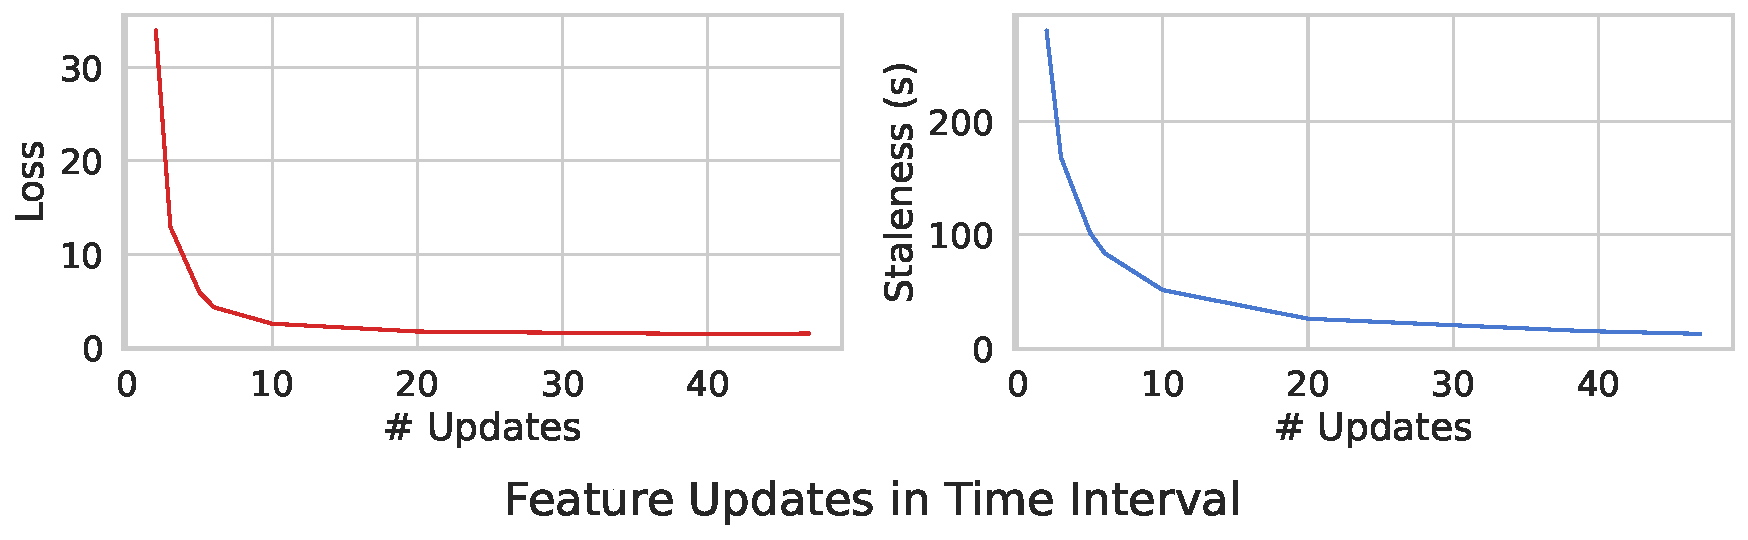
\includegraphics[width=\linewidth]{ralf/figures/loss_staleness_2.pdf}
\centering
\end{center}
 %\setlength{\belowcaptionskip}{-5pt}
 %\setlength{\abovecaptionskip}{-1pt}
\caption{The prediction loss (measured by MASE) on the left is correlated with the feature staleness (time since last update), show on the right. }
\label{f:staleness}
\end{figure}

% \begin{figure}[t]
% \begin{center}
% 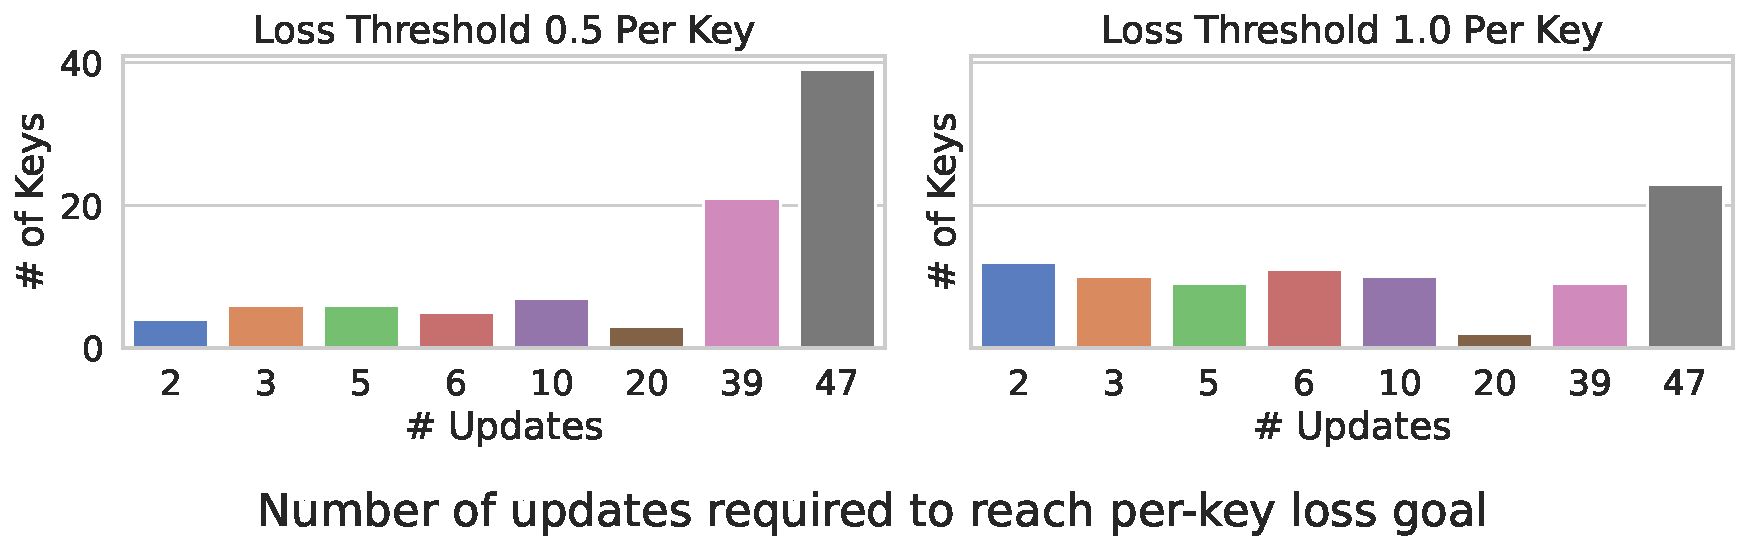
\includegraphics[width=6cm]{ralf/figures/feature_updates.pdf}
% \centering
% \end{center}
%  \setlength{\belowcaptionskip}{-5pt}
% \caption{Distribution of the numbers of feature re-computations required in a time-interval until the accuracy-threshold (0.5 or 1.0) or best accuracy is reached.}
% \label{f:update_variance}
% \end{figure}

% \begin{figure}[t]
% \begin{center}
% 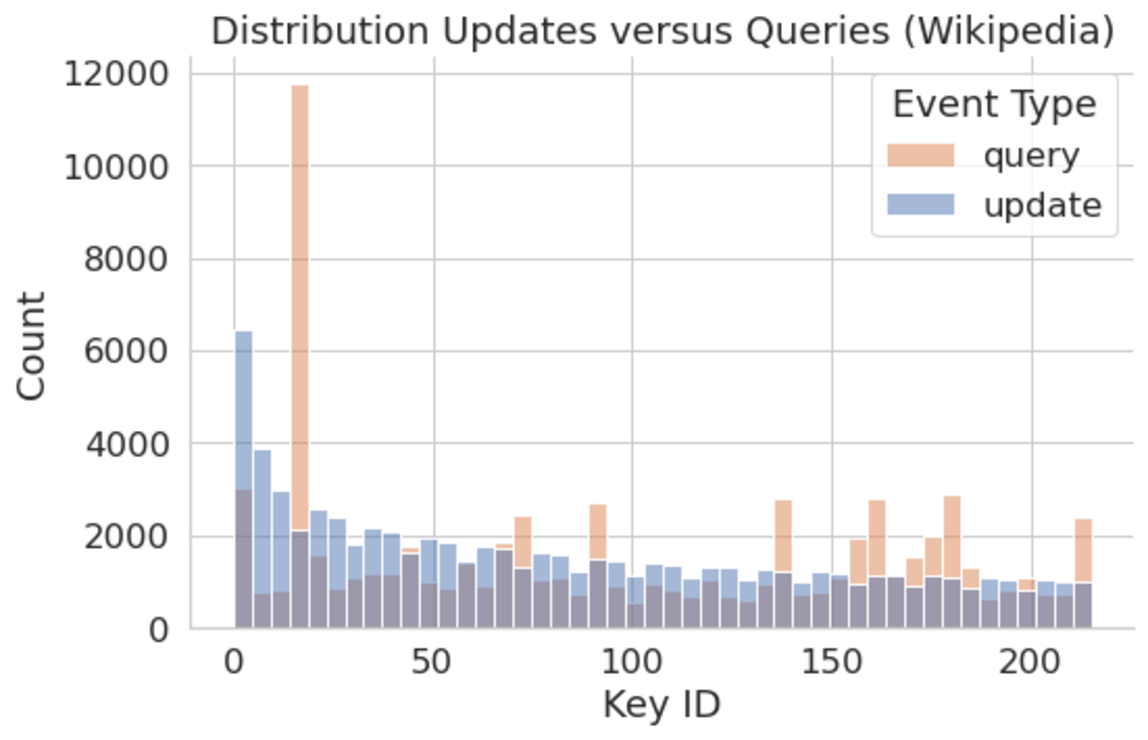
\includegraphics[width=8cm]{ralf/figures/updates_vs_queries.pdf}
% \centering
% \end{center}
%  \setlength{\belowcaptionskip}{-5pt}
%  \setlength{\abovecaptionskip}{-1pt}
% \caption{Distribution of queried keys versus update events to keys for the information retrieval workload (based on Wikipedia document edits and queries collected over a month).}
% \label{f:updates_vs_queries}
% \end{figure}
% \sarah{make figure smaller}
% % %% %---------------------------
% % %---------------------------


% \begin{figure}[t]
% \begin{center}
% 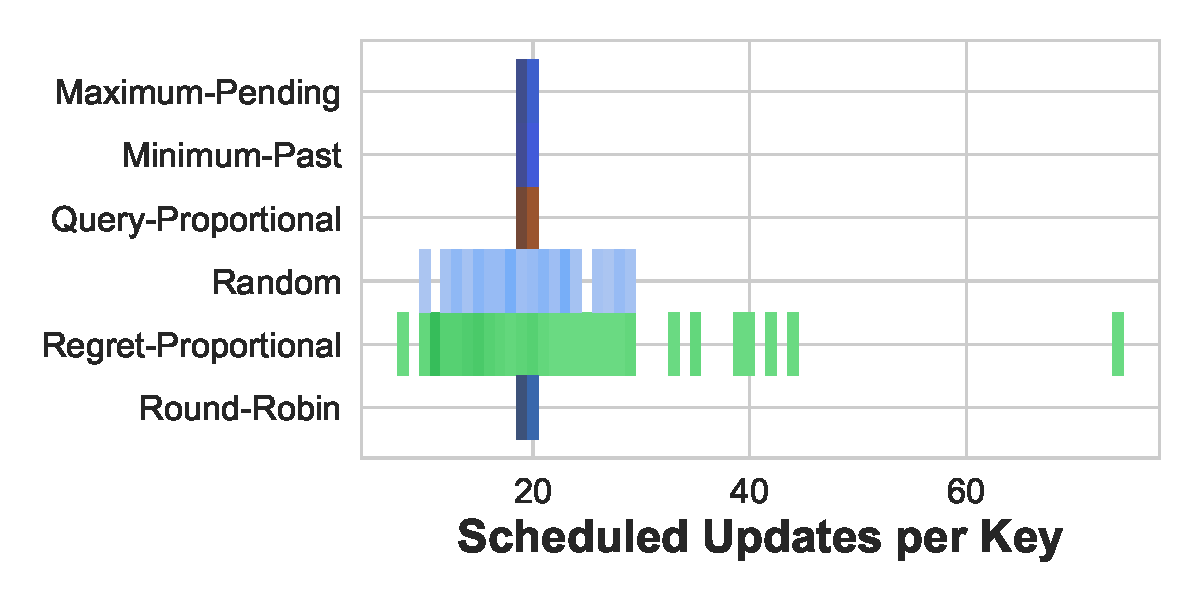
\includegraphics[width=8cm]{ralf/figures/azure_updates_hist_tmp.pdf}
% \centering
% \end{center}
% \setlength{\belowcaptionskip}{-5pt}
% \setlength{\abovecaptionskip}{-1pt}
% \caption{Distribution of featurization updates over keys for baseline (round-robin) versus regret-optimized update scheduling in the anomaly detection workload. Because the rate of raw data updates is uniform across keys, round-robin allocates updates uniformly across keys. The regret-optimize policy is able to non-uniformly distribute updates to reduce downstream error.}
% \label{f:update_variance}
% \end{figure}


% \sarah{recomputations figure: TODO: redo simulation for numbers in this graph bc it looks sus}









%Consider a recommendation model which recommends complimentary products given what a user has already added to their cart. Prior work in prediction serving systems (CITE) would assume that the request-time input is only provided by the query: the products in the cart. However, a real-world model will likely use additional features, such as the user's historical preferences,

%Unlike model training, which is performed relatively infrequently, model inference and pre-processing required features continues to require compute cost for as long as the model is deployed.

% explain more about features!! feature stores. Model serving systems rely on feature stores, contraining features which are expensive to compute. auxilary data. 
% two line starter - get to point. Then go to deeper explanation (look at obladi paper) 

% why is the prioritization unique, or important? we have a clear metric - downstream loss metric that we can compute. in some cases staleness is ok. streaming systems already have a decent amount of studies on deadline. We have a clean way of quantifying how bad the eventual consistency is. 

% Model inference relies on not only prediction input and model weights, but also pre-computed, cached features. Cached features are pre-computed by a separate feauturization pipeline which updates features as new data arrives. Updating features with every data change can be prohibitively expensive when new data is rapidly arriving, and feature operations are compute-intensive. Featurization costs are often controlled by reducing the frequency of re-computing features, resulting in staleness which can impact downstream accuracy. In this paper, we formally define metrics for feature quality in terms of downstream model performance, and introduce policies for optimizing the cost-accuracy tradeoff for maintaining features. 

% In this paper, we study the tradeoff between the compute costs of pre-computing features and the accuracy of the dependent model inference tasks. 


%Machine learning models are increasingly deployed in production to provide personalized and high-quality responses in real-time. 

%Model inference is a core component of many applications, such as e-commerce recommendation and system metric monitoring. Prior work in prediction serving systems (CITE) treats the prediction query as the only input to the model at request time, and the trained model weights as the only parameter impacting prediction accuracy. In reality, model inference relies on additional features generated by a separate featurization pipeline, which typically pre-computes and caches features in a feature store that is queried by the model. The latency of the featurization pipeline can have significant impacts on inference performance, as stale features can degrade prediction accuracy, presenting a tradeoff between featurization costs and downstream model accuracy. In this paper, we explore the cost-accuracy tradeoff of featurization, and develop scheduling policies for streaming featurization using downstream model performance as a metric.  



%
%For example, a model predicting if a user will purchase an item may use an embedding generated from the user's entire history of interactions as additional contextual information. 
%
%


% \textit{Feature Stores} are increasingly becoming a popular design pattern to cache and serve features to models, signifying the need to store pre-computed features. 

%Maintaining features with every new data change is prohibitively expensive, but stale or approximated features can degrade downstream performance. In this paper, we explore the cost-accuracy tradeoff of featurization, and use model inference performance as a metric for evaluating scheduling policies for feature updates. 

%Featurization pipelines are typically separated from inference pipelines, as they are often too expensive to be computed at inference time and must be pre-computed and cached (and models typically have some tolerance for stale features). The latency of the featurization pipeline can have significant impacts inference performance for features which are rapidly changing. 

%Model inference often relies on many different input features, derived with some featurization pipeline. Featurization differs from typical workloads, as features are often pre-computed and cached, and models often have some tolerance for stale features. 



% \textbf{Feature stores signify the need to pre-compute features for low-latency prediction serving systems.}
% Application requirements for real-time predictions constrain the amount of computation that can be done on-request, as inference-time computations must meet tight latency SLOs (CITATION). Real-time prediction serving systems often query an \textit{online feature store} for additional features at inference time. Feature stores are becoming a popular design pattern in industry to enable models to incorporate a features that would be otherwise to expensive to compute. 

% % Models can take advantage of many different features to improve prediction accuracy, such as low-dimentional representations (e.g. embeddings) of additional data. 
% %The need for feature stores come from real-time model serving applications, which must meet tight latency SLOs (CITATION) (<100ms) that constrain the amount of computation which can be performed on-request.
% % Prediction performance depends BOTH the quality of the trained model AND the quality of the pre-computed features. Featurization pipelines should be optimized for downstream model performance.  




% \textbf{Featurization is very expensive - need to determine when to update what }
% \begin{itemize}
%     \item Data updates can be a rapid stream - e.g. user clickstream 
%     \item Updating with every new event is prohibitively expensive - while materializing on-the-fly is too high latency 
%     \item Featurization operators are often not incremental - e.g. computing an language embedding from text that is edited multiple times 
% \end{itemize}

% \textbf{Reducing featurization costs involves accuracy degregation}
% Meeting cost constraints for featurization pipelines often results in performance degredation of the downstream model. A standard protocol to reducing featurization cost is \textit{feature approximation}, where features are approximated by reducing the frequency of re-computation or sub-sampling updates. While models have some degree of tolerance for feature approximation, we find that features which are stale or inaccurate often significantly degrades downstream model performance. As a result, feature maintenance introduces a trade-off between
% \one{} the \textit{cost} of the featurization pipeline, and
% \two{} the \textit{accuracy} of the downstream application performance. 

% \begin{itemize}
%     \item Statistical - not all or nothing 
%     \item Featurization costs are usually reduced by decreasing the frequency of processing feature updates - e.g. dropping updated or increasing window size 
%     \item Models have some degree of tolerance for feature approximation - but eventually performance will degrade  
%     \item As a result, feature maintenance introduces a trade-off between
% \one{} the \textit{cost} of the featurization pipeline, and
% \two{} the \textit{accuracy} of the downstream application performance. 
% %
% \end{itemize}

% Scheduling and load shedding policies for data processing systems used for streaming featurization (e.g. Flink, SparkStreaming) are oblivious to their impact on downsteam model performance. Streaming systems don't natively include mechanisms for adapting to feedback from downstream quality metrics. Scheduling and load shedding policies don't consider the statistical nature of models serving. Defining dependencies between features, as well as between queried features and downstream model performance, is also challenging with existing stream system APIs, making it difficult to propagate feedback on downstream model performance to the correct subset of upstream features. 

% \\
% \\

% % Setup:
% % ML models in complex pipelines that respond to requests in real-time.
% Machine learning models are increasingly deployed in production to provide
% personalized and high-quality responses in real-time.
% %
% The deployment of such models at scale requires the creation of complex pipelines
% which preprocess raw data into \textit{features}, which are fed to a model to generate
% predictions.
% % 
% To meet real-time latency constraints (often <100ms),
% \peter{need citation}
% an emerging pattern in industry combines both streaming and storage systems into a
% \textit{feature store}, which is responsible for serving pre-computed features to models.
% %

% %
% By querying the feature store, models can quickly retrieve features that may be too expensive
% to compute upon request.
% %
% For example, recommendation models may use expensive embeddings that are generated
% from a user's browsing history.
% %
% Querying the browsing history and computing the embeddding at inference time may
% violate tight latency SLOs.
% %
% Instead, the embedding can be pre-computed and cached in a feature store,
% which enables fast responses from the recommendation model.
% %

% %
% Caching introduces the new problem of how features should be \textit{maintained} over time.
% %
% While feature stores may provide fast responses, the returned features may grow
% \textit{stale}, or inconsistent with the latest data.
% %
% Stale features can hurt model performance as they become too out-of-date or miss
% important updates.
% %
% These inconsistencies are especially problematic in the presence of
% \textit{downstream features}, which are features derived from other features,
% because the feature store may serve sets of features which are inconsistent with one another.
% %
% While recomputing features whenever data arrives reduces staleness, these recomputations
% become prohibitively expensive when processing high volume streams or running
% expensive featurization transformations.
% %

% %
% As a result, feature maintenance introduces a trade-off between
% \one{} the \textit{cost} of the featurization pipeline, and
% \two{} the \textit{accuracy} of the downstream application performance. 
% %
% Existing techniques use approximation to reduce cost, but significantly impact accuracy.
% %
% Batching updates (e.g. by assigning updates to a sliding window)
% reduces the frequency of recomputation, but results in stale features.
% \peter{Should mention efficiency, e.g. feeding a batch into a model is cheaper than
% computing one at a time.}
% %
% Sub-sampling updates reduces the number of updates to process, but results in data loss.
% %
% Thus, approximation may reduce the quality of features which may affect the performance
% of the overall pipeline.
% \peter{need citations}
% %

% %
% In contrast, a system can leverage application-level performance metrics to navigate
% the tradeoff between accuracy and cost.
% %
% In this paper, we formalize the problem of feature maintanence as a scheduling problem
% in which updates are scheduled to maximize application performance under cost constraints.
% %
% We evaluate existing scheduling policies for streaming systems in the context of
% feature maintenance.
% %
% We design an adaptive scheduling policy which uses query patterns and information about
% feature dependencies to prioritize updates.
% %
% We evaluate our contributions in
% \textit{Ralf} (\textbf{r}eal-time, \textbf{a}ccuracy, and \textbf{l}atency-aware \textbf{f}eaturization), our prototype featurization pipeline which maintains multiple
% interdependent \textit{feature tables} over streaming updates.

% The rest of the paper is organized as follows:
% \peter{TODO: fill this in with summaries of each section}


% Machine learning models are increasingly being deployed the serve predictions in real-time. Real-time serving systems are often subjected to tight latency constraints (<100ms), limiting the amount of data retrieval or computation that can be done when a prediction is requested. A common design pattern in industry machine learning pipelines is to deploy a \textit{feature store}, responsible for storing and serving pre-computed features to models. 

% fundamental question - how should data changes to propagated? or given that some parts of a computation can be cached, have varying latency, etc. how can we schedule maintenance? 

% Data processing steps in ML pipelines are also typically expensive (such as aggregations over large amounts of data, or model predictions) 
% two questions: what should be materialized, and what should be cached - OR just the question - what upstream updates should be materialied when 
% Updates to raw, upstream data sources must propagate to downstream, derived data, known as "features". 

% How are features computed? Why are we compute-bound? Introduce notion of accuracy to
% optimize compute.
% Features are typically computed either
% \one{} \textit{eagerly} where raw data is immediately processed into features, or
% \two{} \textit{lazily} where features are generated in response to a query.
% %
% Eager computation ensures low-latency responses at the cost of more resources,
% whereas lazy computation uses just enough resources to respond to queries but may
% result in higher response times.
% %
% While eager computation may meet the latency constraints of real-time machine learning
% pipelines, the resource intensive nature of machine learning workloads may be
% prohibitely expensive.
% %
% Thus, feature stores need to pursue a best-of-both-worlds approach and identify
% high-priority features to compute eagerly to ensure low response times,
% and lazily processing low-priority features to reduce costs.
% %
% 
% %
% Choosing which features to compute eagerly introduces new challenges related to
% feature \textit{maintenance}.
% %
% Features derived from high volume data streams, such as e-commerce clickstreams
% or system logs, constantly receive new data.
% %
% \textit{Downstream features}, which are derived from previously-computed upstream features,
% grow stale and may affect overall pipeline performance if features become too out-of-date
% or miss important updates.
% %


%
% Pre-computed, cached features allow real-time models to query for contextual features at inference time which would otherwise be too expensive to compute on-request. For example, a model predicting if a user will purchase an item may use an embedding generated from the user's history of interactions as an additional feature. Querying the user's historical data and calculating the embedding at inference time could violate tight latency SLOs. Instead, the embedding can be pre-computed and cached in a feature store, so the model can query the user's embedding when making a prediction. 

%The feature store is responsible for versioning features to ensure feature transformations are used across training and inference time, and responding to feature query requests with sufficiently low latency (usually through storing features in an in-memory database). 

% Caching features introduces new challenges. Slight changes to the featurization transformations can cause dramatic performance degregations for downstream model predictions due to data drift, unless the model is re-trained with the new version of the features. Features are often generated from upstream data sources, which may be rapidly changing (such as with streaming data sources). Features need to be maintained by processing upstream updates. However, re-computing features for every new update can be prohibitively expensive for high-density streams of updates running through expensive featurization transformations. 

% Caching features introduces the problem of how cached features should be \textit{maintained} with new data. Features derived from data streams, such an e-commerce clickstream or system logs, are constantly receiving new data. As new data arrives, downstream features grow stale, and can hurt downstream model performance if features grow too out-of-date or miss important new updates. However, re-computing features for every new update can be prohibitively expensive for high-density streams of updates running through expensive featurization transformations. 

% Existing streaming featurization pipelines reduce compute costs with feature "approximation", such as by batching or sub-sampling updates. Batching or windowing updates reduces the frequency of re-computation, but results in staler features depending on the window size or the time between batches. Sub-sampling updates reduces the number of updates that need to be processed, but results in data loss. Approximation can reduce the quality of features and degrade downstream performance, as features will be less fresh or missing data. 

%In addition, processing upstream updates it not always beneficial, such as if the feature being updated is never queried, or if the feature is unlikely to change. 

%Caching features introduces the problem of how cached features should be \textit{maintained} with new data. The raw data sources which features are derived from are often rapidly changes, such as in cases where features are derived from aggregating over data streams. Features are generated from transforming one or more upstream data sources (or even other features). Updates to upstream data should be propagated to be reflected in downstream features by re-computing the features with the new data. However, re-computing features for every new update can be prohibitively expensive for high-density streams of updates running through expensive featurization transformations. 

% \begin{figure}[t]
% \begin{center}
% \includegraphics[width=8cm]{ralf/figures/fake graph.png}
% \centering
% \end{center}
% \caption{\label{fig:vectors} Feature store overview. }
%     \label{f:feature-store-overview}
% \end{figure}



%Despite the importance of features for downstream model performance and the significant cost of feature updates, there are few policies for scheduling feature updates. 



% As a result, feature maintenance introduces a trade-off between (1) the \textit{cost} of the featurization pipeline, and (2) the \textit{accuracy} of the downstream application performance. Managing this tradeoff is an unexplored problem, and current featurization pipelines lack metrics to provide feedback on feature quality. Existing metrics for optimizing schedulers for data streaming or query processing are insufficient for featurization pipelines, which ideally should be optimizing for performance of the downstream task. Associating upstream data updates and downstream queries is difficult without clear dependencies defined between features, which can be defined in terms of multiple other data sources and features.



%Existing metrics for optimizing schedulers for data streaming or query processing are insufficient for featurization pipelines, which ideally should be optimizing for performance of the downstream task. Feature stores may contain multiple interdependent features which all require varying degress of freshness. 

% interdepe


%Most feature stores focus on the data drift challenge through versioning features, managing feature metadata, and synchronizing features used in training and inference pipelines,  


%Features computations are often high latency and compute intensive. For example, a user preference embedding may require querying a user's entire history of interactions and running the history through an expensive embedding model. For such features to be used for online predictions with tight latency constrains, the features must pre-computed and cached. Cached features must still be updated with underlying data changes, such as new user interactions. However, re-computing features for every new event can be prohibitively expensive. Featurization costs are typically reduced by approximating features, such as by reducing the frequency of re-computation, such as with windowing, batching, or sub-sampling updates. Approximation can reduce the quality of features and degrade downstream performance, as features will be less fresh or missing data. 

% Our work introduces a featurization pipeline which is both quality and query aware to maximize downstream inference performance. In this paper, we make the following contributions: 
% \begin{itemize}
%     \item We formalize the problem of feature maintenance in terms of maximizing downstream application performance under cost constraints.
%     \item We evaluate existing load shedding and prioritization policies for streaming systems in the context of feature maintenance. 
%     \item We design an adaptive scheduling policy which uses query pattern and feature dependency information to prioritize updates.
%     \item (Learned scheduler thing?) 
%     \item We build a prototype featurization pipeline, \textit{Ralf} (realtime, accuracy and latency-aware featurization), which maintains multiple interdependent \textit{feature tables} over streaming updates. Ralf tracks update and query patterns over feature keys to propagate to schedulers.  
% \end{itemize}
% 


%%%%%%%%%%%%%%%%%%%%%%%%%%%%%%%%%%%%%%%%%%%%%%%%%%%%%%%%%%%%%%%%%%%%%%%%%%%%
% BACKGROUND
%%%%%%%%%%%%%%%%%%%%%%%%%%%%%%%%%%%%%%%%%%%%%%%%%%%%%%%%%%%%%%%%%%%%%%%%%%%%
\section{Background}
\label{s:background}

\begin{figure*}[t]
\centering
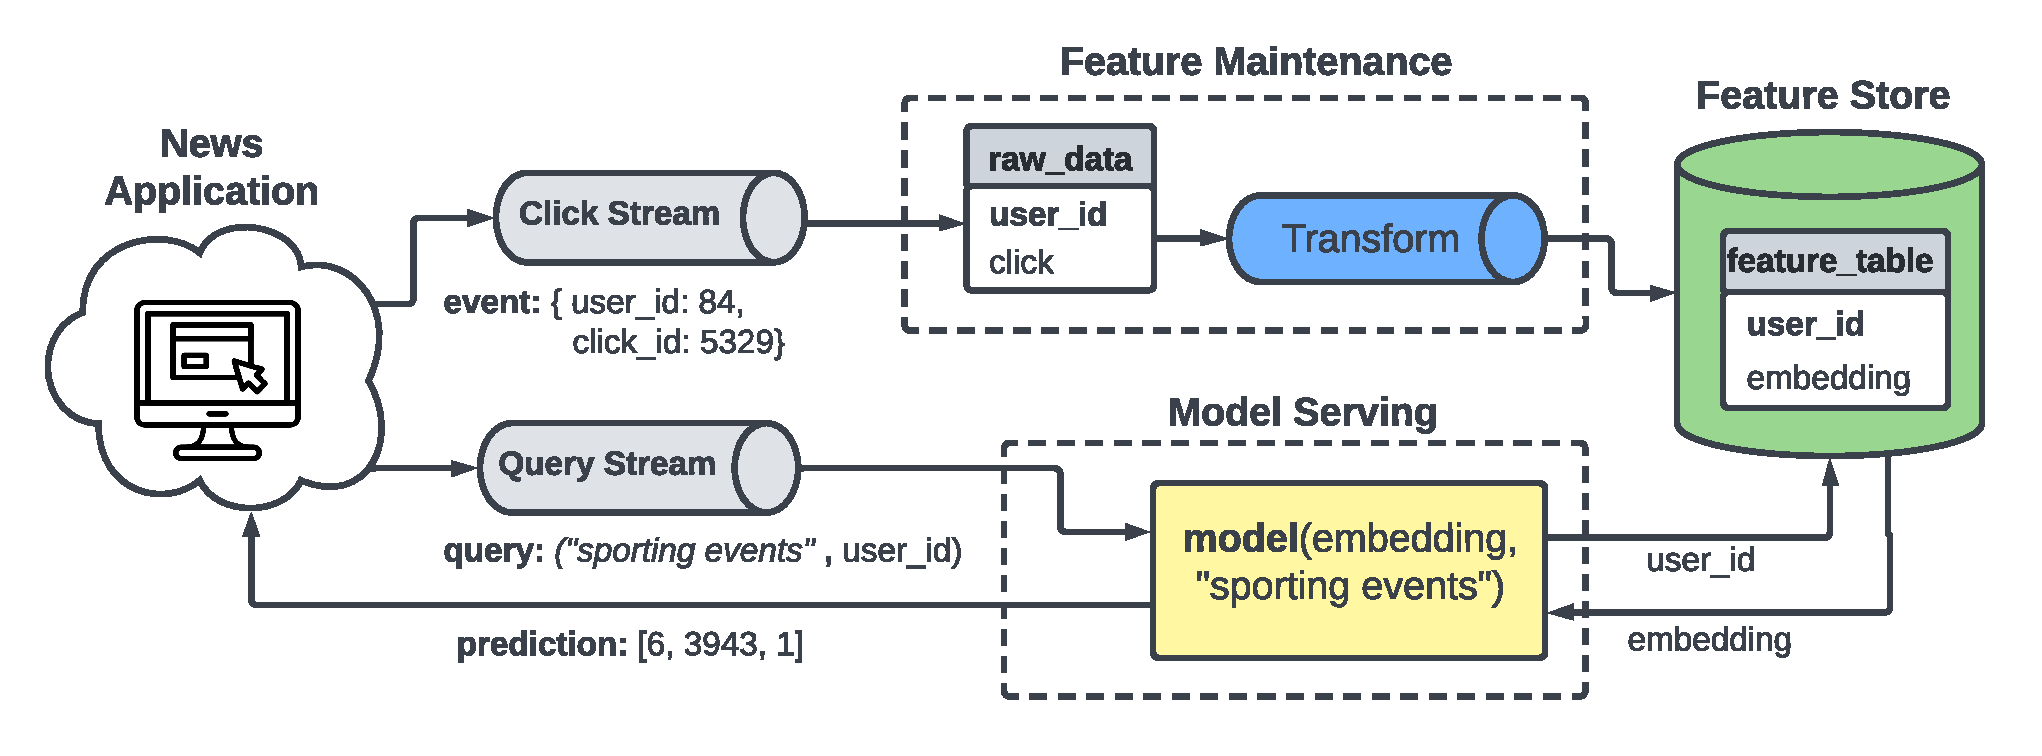
\includegraphics[width=14cm]{ralf/figures/feature_store.pdf}
%\setlength{\belowcaptionskip}{-10pt}
%\setlength{\abovecaptionskip}{10pt}
\caption{A ML serving pipeline with a feature store. 
%for a news application logging user clicks (\textit{click/event stream}) and submitting queries to a model when the user makes search requests (\textit{query stream}). 
%The model looks up the user's embedding, derived from historical click data, as an additional input to make a prediction (e.g. a list of recommended article IDs). 
}
\label{f:feature-store}
\end{figure*}

Most machine learning applications rely on \emph{features} to summarize relevant aspects of the training data and provide the necessary context to make informed predictions.
To illustrate, we return to our 
online news recommendation service example (\S\ref{s:introduction}). 

In this setup, the model $m$ must predict the probability $\hat{y}$ that user $u$ will click on article $a$ given a search query $x$.  
Most papers in the area will denote this seemingly simple prediction task as
\begin{equation}
    \hat{y} = m(x, u, a).
\end{equation}
 \amit{Papers in the machine learning and systems community often advance methods to design, train, and efficiently compute the model $m$. In this paper, however, we focus on how to compute the features $u$ and $a$ to optimize accuracy.} \joey{I don't know if we need this change here did the reviews not like the informality of the writing.} \amit{R3 said "Also, the authors should tone down this overstatement: ”After all, most papers in the machine learning and systems community are about how to design, train, and efficiently compute the model m.”"}
 After all, most papers in the machine learning and systems community are about how to design, train, and efficiently compute the model $m$. 
In this paper, we focus on how to compute the features, $u$ and $a$, to optimize accuracy. 

Hidden in this notation is the need to transform \textit{historical data} associated with the user $u$ and article $a$ into their respective features, which can encode everything from the user's entire click history, to the contents of the article, and even the histories of other users that clicked on that article.
As a consequence, a more accurate notation for this task would be:
\begin{equation}
    \hat{y} = m\left(x,
    f_\text{users}\left(\mathcal{D}^{t}_u\right), 
    f_\text{articles}\left(\mathcal{D}^{t}_a\right) 
    \right), 
\end{equation}
where the functions $f_\text{users}$ and $f_\text{articles}$ are \emph{featurization functions} and $\mathcal{D}^{t}_u$ and $\mathcal{D}^{t}_a$ are all the data up until the present ($t$) that is associated with the user and article.
Each of the feature functions returns a vector that is combined with the query text $x$ and processed by the model $m$. $m$ makes a prediction, calculating the probability that user $u$ will click the article $a$.

While the aforementioned example described only a couple of features, in practice, there may be dozens of features from different data sources computed for a single prediction. Automated feature generation tools make is easy to generate hundreds of unique features from data \cite{feature-tools}. For notational simplicity, in this paper we will focus on a single featurization function $f$ and key $k$:
\begin{equation}
    \hat{y} = m\left(x, 
    f\left(\mathcal{D}^{t}_k\right)
    \right). 
\end{equation}
where $x$ is the query and $\mathcal{D}^{t}_k$ is the historical data for key $k$. 
%\natacha{Should we make it explicitly clear here that we are therefore assuming that the features are independent from each other? I don't think we have explicitly stated this assumption anywhere}
% However, the techniques we introduce apply to settings with additional feature functions. 
% \joey{maybe drop the last sentence.} \natacha{grammar}\joey{yep.}

Querying available historical data $\mathcal{D}^{t}_k$ and computing the featurization function $f$ for each prediction request may be prohibitive in low-latency prediction serving settings where recommendations must be generated in real-time a users are scrolling through their news feed.
% \natacha{note, this suggestst that there's two issues, the large data size, and the cost of th function. is that true?} \joey{yes, we probably should actually address each part separately and in this paper we sort of side step the access costs and focus on computation.  Possibly a mistake.}
Each query may need to access large amounts of historical data and run a computationally expensive feature function $f$. For example, many recent content recommendation models employ deep learning techniques to encode click streams and article contents and run online gradient descent~\cite{DLRM19}.
%

Furthermore, many predictions may query the same keys, resulting in redundant computation. Often the same user features will be used to rank multiple articles and the same article will be ranked for many users. Executing the query on the entire history of users and articles for each new prediction is redundant, expensive, and infeasible for latency constrained settings.

% For the prediction serving application to generate features for some key $k$ when a prediction query is made, the application needs to lookup the current $\mathcal{D}^{t}_k$ available for key $k$ from some data table, \texttt{historical\_data}. We can represent the SQL query the prediction serving application makes for features as: 
% \begin{lstlisting}[
%           language=SQL,
%           basicstyle=\ttfamily,
%           numberstyle=\tiny,
%           commentstyle=\color{gray}, 
%           label={lst:select}
%         ]
%     SELECT key, f(data) 
%     FROM historical_data WHERE key=k
% \end{lstlisting}
% where $f$ is the feature function implemented as a UDF. However, the latency of this query may be prohibitive in low-latency prediction serving settings where recommendations must be generated in real-time as as users are scrolling through their news feed. 



To guarantee low-latency feature queries and avoid redundant computation, features are often \textit{pre-computed} and stored in low-latency data store, referred to as \textit{feature stores}. 
% in industry ML pipelines. 




\subsection{Feature Stores}
The \emph{feature store} is a nascent class of systems which target the problem of storing and maintaining feature tables. We show an overview of a how feature stores, model serving, and applications interact in \cref{f:feature-store}. There are several major open-source and commercial feature store systems \cite{featurestoresorg,tecton, hopsworks, amazon}. Feature stores can be used to fulfill a variety of requirements, such as enabling sharing of features across different multiple downstream applications, improving latency and cost by pre-computing features, and managing metadata about features (e.g. version control), which we discuss further in Section ~\ref{s:discussion}. In this paper, we focus specifically on maintaining feature table over streaming data updates in the context of online prediction serving. 

% To eliminate the need to run expensive feature computation when serving low-latency predictions, it is common practice to pre-materialize features and store the values in a \emph{feature table} that is stored in a low-latency data store.  
% The feature table is essentially a materialized view over raw, historical data. Pre-computing feature table values eliminates redundant computation across multiple predictions, and helps meet prediction latency constraints.  feature values can be reused across multiple predictions. 
% \begin{lstlisting}[
%           language=SQL,
%           basicstyle=\ttfamily,
%           numberstyle=\tiny,
%           commentstyle=\color{gray}
%         ]
% CREATE MATERIALIZED VIEW feature_table 
% AS (
%     SELECT key, f(data)
%     FROM historical_data
%     GROUP BY key
% )
% \end{lstlisting}
% \natacha{This might not be the right place yet, but we've not discussed at all the consistency requirements}
%\subsubsection{Feature Maintenance}

% The feature table can be fully refreshed when enough new data is recieved, or we can also update a specific key $k$ with inserts like the following:
% \begin{lstlisting}[
%           language=SQL,
%           basicstyle=\ttfamily,
%           numberstyle=\tiny,
%           commentstyle=\color{gray},
%           escapechar={|}
%         ]
% INSERT INTO feature_table(key, value) VALUES
% (
%     SELECT key, f(data)
%     FROM historical_data
%     WHERE key = |\color{red}{k}|
% )
% \end{lstlisting}

As the underlying, raw data is updated over time, pre-computed features need to be \textit{maintained} to prevent feature staleness, which may degrade prediction quality of dependent downstream models. For example, a feature encoding a user's interests in news topics can change rapidly with each new action by that users. If the feature is not updated over time, the stale encoding may degrade the quality of recommendations made by a model for that user. 

Existing feature store typically rely on external data processing systems (e.g. Spark, Flink) to compute feature updates from new data. These systems then process new data in either a streaming or batch fashion to update current feature values.


\subsection{Feature Maintenance}
Maintaining features with new data can be computationally expensive, depending on the rate of new data arrival, the cost of the featurization function, and the required feature freshness.  While some feature functions can be incrementally applied to new data, many require significant re-computation over a large window of historical data with the arrival of each new record.   
For example, an attention-based text document embedding model will need to re-compute the embedding of the entire document to reflect a single word change. \jmh{give a canonical citation}
\joey{Kevin, maybe we can reference the colBERT paper here?}
Even when feature functions can be applied incrementally, running them in a streaming fashion on high velocity data streams can require expensive computational resources (e.g., GPUs) and be less efficient than large batch updates~\cite{clipper, crankshaw2020inferline}. 


Updating features with every data change can be expensive and unnecessary, depending on how quickly the true feature value is changing and how much impact staleness has on model predictions. In cases where models are robust to stale features, running a daily batch job to process new data is sufficient. In other cases where models are sensitive to feature staleness, features may need to be continuously updated with new data. For example, Splunk uses Flink for streaming maintenance of time-series features for real-time anomaly detection \cite{mishra2021onlinestl}, and has developed application-specific solutions for maintaining fresh features for high cardinality data streams \cite{mishra2021onlinestl}. 
Feature values are typically \textit{eventually consistent} with respect to the underlying raw data.
% \sarah{is this a correct use of the term "eventually consistent"?} \joey{Yeah close enough.}



To provide a specific example, we implement a workload similar to Splunk's in Flink where we maintain a time-series decomposition for a set of cloud virtual machines, each streaming CPU utilization data. Updating a feature for a given virtual machine (i.e. the key) takes about 0.3 seconds, so a single Flink process can only update about 3-4 features per second. Existing systems do not natively have application awareness to prioritize updates, so will use a FIFO queue to process new data in incoming order. As a result, increasing the cardinality of the dataset eventually results in the per-key staleness linearly increasing with time as updates 
lag
% fall further and further behind 
new data, as shown in \cref{f:flink}. These increases in feature staleness are correlated to decreased prediction accuracy, as shown in \cref{f:staleness}.

% %Real-time maintenace can be paticularly challenging when there is a high-rate of incoming data (e.g. high-density clickstreams) and high cardinality (e.g. features for millions of users), requiring a large number of updates to process to maintain fresh features. 
% The increasing importance of maintaining fresh features in the face of these challenges has motivated a number of workload-specific solutions. Tecton has released a blog post citing cost as a barrier to high feature freshness \cite{tectonfreshness} and developed new methods for computing real-time aggregation windows more efficiently \cite{tectontile}. \kevin{This seems a bit outdated to me and I think we can remove it} Splunk faced challenges with featurizing high cardinality data streams with time-series decomposition for downstream anomaly detection models  \cite{mishra2021onlinestl}, motivating development of an online time-series decomposition algorithm. 

In this paper, we show that scheduling feature updates according to each key's impact on downstream accuracy allows us to preserve overall accuracy at lower cost. Feature stores %are uniquely situated between updates to features and feature queried, but 
typically lack awareness of downstream query patterns and performance of the predictions made using queried features. As a result, systems for maintaining features treat all data updates and keys symmetrically and fail to leverage important information about which updates are critical and which keys are likely to be accessed in the downstream prediction workload. 



%Many real-time applications such as recommendation or anomaly detection systems benefit from features which provide \textit{real-time context}. These features are derived by transforming real-time data streams, such as user clickstreams. 

%While more machine learning pipelines move towards leveraging real-time data \cite{chip}, these pipelines struggle to support to support complex streaming transformations (e.g. model predictions) while also maintaining high freshness, especially for high cardinalities. Many recent ML models (e.g. sequence/text models) have high CPU inference latency \cite{huggingface}. Furthermore, high cardinality feature tables (e.g. features for millions of users) may need to simultaneously process updates to many keys concurrently, even if the individual update rate for each key is small. 

% https://blog.roblox.com/2020/05/scaled-bert-serve-1-billion-daily-requests-cpus/
% https://arxiv.org/abs/2102.06621
% https://huggingface.co/blog/bert-cpu-scaling-part-1#4-out-of-the-box-results




\sarah{(TODO: R5. Add a discussion on real world scenarios in which one cannot update all features in time.}
\joey{I think what is here is not bad. I spent some time looking for papers that describe slow feature computation but its hard to find since feature cost is not typically a focus of ML.}

% \textcolor{red}{
% \subsection{Sustaining Expensive Features}
% }
% \textcolor{red}{In cases where the incoming data rate exceeds the throughput of the data processing, the written features will become stale as the data processing engine falls behind. We implement in Flink one of our evaluation workloads (described in SECTION) for maintaining time-series information per cloud VM CPU logs.   Existing systems do not natively have application awareness to prioritize updates, so will use a FIFO queue to process new data in incoming order. We show in \cref{f:flink} how this results in increasingly staleness as the cardinality of the incoming data stream increases. These increases in feature staleness are correlated to decreased prediction accuracy, as shown in \cref{f:staleness}}.

\begin{figure}[t]
\centering
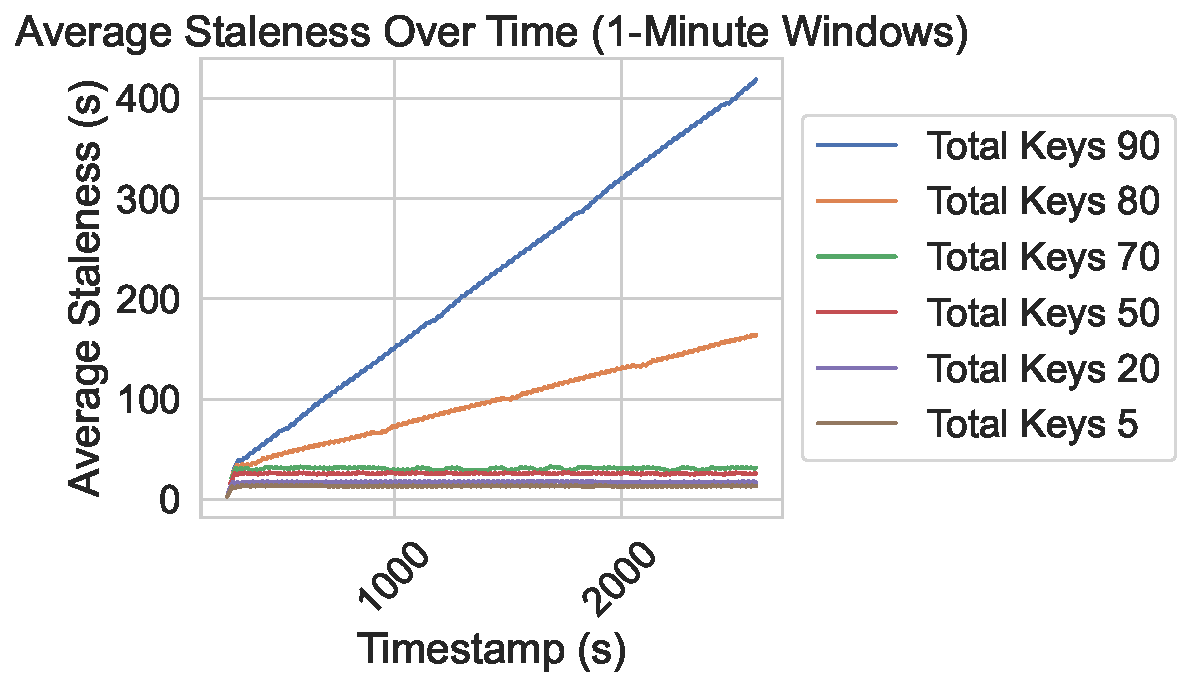
\includegraphics[width=7cm]{ralf/figures/flink.pdf}
\caption{Average staleness in a 1-minute time window across all keys as a function as the cardinality.}
\label{f:flink}
\end{figure}


\sarah{The full Azure dataset has 2 million keys producing data once every 5 minutes, which on lambda  (\$1.7xe-5 per GB-second) would cost \$5,175/day without including data query time. Even supporting 6k active users each producing 10 events/minute costs \$1440/day. Reducing the rate of re-computation naively results in accuracy degradation as shown in Fig 8, 11, and 13.} \amit{We can even specify that this is still a really small use case -- most companies doing some kind of featurization will at least have ~hundreds of features per user, so with a 1M MAU and features calculated every hour on average, it would be cost prohibitive to update.}


%\subsubsection{Consistency Requirements} 
%\textcolor{red}{Reference weak consistency literature from Natacha.} Consistency requirements for feature tables vary across applications and types of features.
%How quickly feature values change over time, and how much they impact downstream model training and inference applications, can significantly vary across different types of features. In cases where models are robust to stale features, running a daily batch job to process new data is sufficient to keep feature up-to-date. In other cases where models are sensitive to feature staleness, features may need to be continuously updated with new data. For example, Splunk uses Flink to maintain time-series features used for anomaly detection \cite{mishra2021onlinestl}. Choosing the frequency of feature updates depends on the cost of featurization, the rate of new data arrival, and the sensitivity of models to staleness. 
 
\subsection{A Feature Store Reference Model}
For simplicity, we first describe the standard formulation of a feature store. 
In Section~\ref{s:discussion}, we discuss the full variety of feature stores presently being used, and how our work applies.

We assume that raw historical data is loaded into a data warehouse, capturing the basic entities (users, movies) and actions (users seeing ads, users viewing movies, etc) we use in prediction. We then consider a derived \emph{feature table} that memoizes \emph{featurization functions} over that data. This table can also be stored in the data warehouse, or it can be maintained in an external cache database like Redis or Memcached; our design does not depend on that decision. A SQL query that populates the feature table exhaustively would have a template that looks like this:
\begin{lstlisting}[
           language=SQL,
           basicstyle=\ttfamily,
           numberstyle=\tiny,
           commentstyle=\color{gray}
        ]
    SELECT key, uda(data)
    FROM historical_data
    GROUP BY key
\end{lstlisting}
where \texttt{uda} is a user-defined aggregate function. If the feature store is kept in the warehouse, feature tables can be viewed as traditional materialized views. 
%it could be represented as a materialized view of the full featurization query.
\jmh{I think some of the discussion here is using a naming scheme that got lost in copying. I think I labeled the query above as ``the featurization query'' (without the materialized view aspect), and the alternative below the ``cache maintenance query'').}
\natacha{Temporarily removed Joe's text for consistency}
Materialized views, however, are typically kept consistent with underlying data, and must be recomputed on every new update. Systems that support incremental view maintenance incur similar costs when the supplied feature function cannot be recomputed incrementally. In contrast, \system{} focuses on carefully choosing when and what keys to recompute to minimize resource costs while preserving accuracy:
\begin{lstlisting}[
           language=SQL,
           basicstyle=\ttfamily,
           numberstyle=\tiny,
           commentstyle=\color{gray},
           label=lst:cache-maintenance
        ]
    SELECT key, uda(data)
    FROM historical_data
    WHERE key IN <PolicyQuery>
    GROUP BY key
\end{lstlisting}
%Our focus in this paper is the design and execution of this maintenance query—particularly the design of the inner "policy query" and the schedule for running the outer Cache Maintenance query
The fundamental policy decision addressed in this paper is: \emph{given the above query can only be run on a small subset of all possible keys at a time \amit{due to cost constraints},
which keys do we select to ensure maximum downstream prediction accuracy. }
\natacha{two issues to me here 1) we're not focused on the design of the query, we're focused on when we choose to execute the query. Second, what's the cache maintenance query? first time we mention it. Old version in text please feel free to add back} We focus on making scheduling decisions across keys (rather than between updates pertaining to a single key), as large key cardinality is a common attribute in feature store applications. We use SQL here to illustrate our ideas, but of course this logic could be implemented in a number of scalable data-centric APIs, including Spark, Flink, and so on.
\sarah{Link back to PolicyQuery in later sections}

\natacha{It felt a little strange to introduce SQL out of nowhere given it's not something you really discuss aywhere else in the paper, etc. Could you do without? Formulating it as a materialized view problem makes sense, it was specifically the sudden "here's SQL code" that was strange to me} 
As we discuss in Section~\ref{s:discussion}, there are many options for materializing and storing features. Our simple model here is designed to be sufficient to illustrate the key policy issues at hand; further architectural complexity is discussed in Section~\ref{s:discussion}.

%%%%%%%%%%%%%%%%%%%%%%%%%%%%%%%%%%%%%%%%%%%%%%%%%%%%%%%%%%%%%%%%%%%%%%%%%%%%
% FEATURE QUALITY
%%%%%%%%%%%%%%%%%%%%%%%%%%%%%%%%%%%%%%%%%%%%%%%%%%%%%%%%%%%%%%%%%%%%%%%%%%%%
\section{Efficient Feature Maintenance}

In this section, we formalize the feature maintenance problem addressed in this paper, that is, selecting the keys for \cref{lst:cache-maintenance}. 
In a resource-constrained setting, only a subset of features can be updated at any given time, resulting in feature staleness which may degrade prediction accuracy. The focus of this paper is precisely to optimize this issue: deciding which keys to update in response to new data, with the objective of maximizing downstream prediction accuracy. As previously highlighted, the core enabling factor is the differentiated impact that feature staleness has on overall accuracy: stale features may lead to low query errors, while some features may simply rarely be queried at all. \amit{different features will have different impacts on downstream accuracy, as some features might rarely be queried whereas others might contribute significantly to the model's output.}
\jmh{Next sentence needs grammar fix, and should be an echo of the intro! If you find yourself typing "this is the focus of the paper" in Section 3 it means you're concerned that Section 1 failed to do its job. "\emph{The focus of this paper is precisely to optimize this issue: deciding which keys to update in response to new data, with the objective of maximizing downstream prediction accuracy.}"}

\natacha{This paragraph felt a little strange as you've already said this multiple times in S1 and S2, but you've written it in a way that makes it sounds like it's new information. I added three lines and vote to remote the rest of this paragraph. TEMPORARILY COMMENTED OUT}
%The impact of feature updates on accuracy can vary with the query distribution over features and the the impact of the new data on the current feature value. In some cases, the frequency of data changes may be uncorrelated with the query pattern from downstream applications, resulting in frequent updates to keys that are seldom queried, as show in \cref{f:updates_vs_queries}. Even for features queried with similar patterns, the importance of incoming data updates may vary. Some updates may radically change predictions; others may have little impact on predictions and can be deferred or ignored. 
%For example, the first few comments on an article can have a significant impact on the rating of that article. In contrast, later comments may have a negligible impact in downstream prediction accuracy. Similarly, largely redundant or uninformative comments on an article are unlikely to affect user preferences.
%


%At the same time, there is more flexibility \jmh{more than what?} with how features are maintained \natacha{Compared to what?}. In contrast to traditional caches that must fully invalidate entries with changes in the data, stale features have the \emph{potential} of negatively impacting accuracy.  \natacha{For what it's worth, I never really thought of features as caching, more thought of them as a materialization, so this sentence didn't resonate with me a lot}






% Furthermore, we have a clearly defined objective of minimizing the impact of inaccurate features on the downstream prediction accuracy. 
% \natacha{The last three sentences seem strewn together but don't seem to follow logically from one another}


\natacha{It would be cool to have a separate section that makes a bigger deal out of this, right now it's a little lost in everything else. We know how hard staleness and weak consistency is to deal with, but now we have a solution! We can actually numerically assess what the true cost of weak consistency. It's huge!}



\subsection{Feature Approximation} 
\label{sec:approximation}
%The cost of feature maintenance can be reduced by introducing approximation to the way the feature values are maintained. 


%Calculating $v^t_k$ at each timestep for all keys is often prohibitively expensive, necessitating that feature values are approximated with some $\tilde{v}_k^t$. We can approximate $\tilde{v}_k^t$ by approximating the featurization (e.g. with data sub-sampling \cite{wedge2018solving} or using a lighter-weight feature function \cite{willump}), or by using past (stale) version of the feature value. In this work, we focus on the latter mechanism by choosing what keys to update and what keys to keep the stale values for. 

%\subsubsection{Stale Features} 
Featurization cost can be reduced by computing features using approximated featurization (e.g. sampling) or using stale features, which is the focus of this paper. Reducing the frequency of updating feature values by tolerating staleness is a simple way to reduce featurization cost, as the same update function can be used on the same data: the only parameter to change is when the update is triggered. For example, multiple edits to a document can be batched together so the document only needs to be re-embedded once, or a function over a window of data can be run less frequently to reduce computational cost. 


For feature derived from data $\mathcal{D}^{t}$, we denote the true feature values at time $t$ as $v^t_k = f\left( \mathcal{D}^{t}_k\right)$, and the stale feature values as 
\begin{equation}
    \tilde{v}^t_k = f\left( \mathcal{D}^{t-\delta_{k,t}}_k\right).\label{eqn:delayedupdate}
\end{equation}
% We formally denote the approximation achieved by delaying updates as: 
% \begin{equation}
%     \tilde{v}^t_k = f\left( \mathcal{D}^{t-\delta_{k,t}}_k\right).\label{eqn:delayedupdate}
% \end{equation}
where $\delta_{k,t}$ is the staleness of the current feature value.  Delaying update processing, and thereby increasing the staleness, reduces how often $f$ needs to be run on new data. However, reducing the frequency of re-computation results in features that are more stale, as entries in the feature table are more likely to be missing the most recent updates. 

\subsubsection{Evaluating Approximation Quality} Standard ways to evaluate the quality of approximation is to evaluate the staleness of the queried data, or the differences in the approximated and unapproximated value. However in the context of feature stores, these metrics do not necessarily correlate to prediction quality. Feature staleness or large divergence in feature values is not problematic if the prediction quality is not impacted. Similarly, slight changes in the feature values can dramatically change predictions\sarah{try to cite something}. For example, neural networks can be very sensitive to small perturbations in input, and it is difficult to model how differences in feature values will correlate to differences in predictions, especially when the input values to the model are unknown.  \sarah{try to cite something}

However, directly using downstream accuracy as a metric for feature quality is problematic, as prediction quality depends on \textit{both} the features and the model. A model may perform poorly for an out-of-distribution user regardless of feature approximation quality. In order to disentangle model performance from feature quality, we propose \textit{feature store regret} in the next section. 

%We can denote approximate feature updates as:
%\begin{equation}
%    \tilde{v}^t_k =  f\left( s(\mathcal{D}^{t}_k)\right).\label{eqn:sampling}
%\end{equation}
%where $s$ is some sampling function that takes all the available data $\mathcal{D}^{t}_k$ at time $t$ and returns a subset of that data.
%Because feature computation often depends linearly or polynomially in the data size, sampling can significantly reduce computational costs often without significant impact on the feature store loss.



%In \cref{eqn:delayedupdate}, we delayed updates uniformly.  
%However, in practice we may choose to assign a separate delay $\delta_k$ for each key or even make the delay a lightweight function of $\delta(\mathcal{D}^t_k)$ of the data associated with that key.
%By prioritizing keys that are more likely to be accessed we can ensure that those keys will have more up-to-date features.
%In many settings, we would expect the query access pattern for features to be relatively stable providing strong signal for which keys are likely to be accessed in the future.

%Furthermore, not all data will result in significant changes to the feature values.  
%Therefore, we can prioritize updating features that have significant new data.


% \begin{figure}
% \centering
% \begin{subfigure}[b]{0.5\textwidth}
%    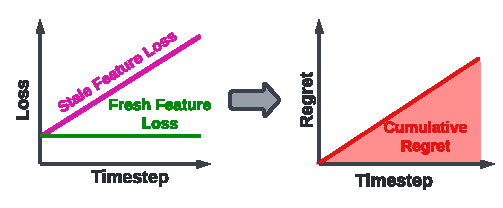
\includegraphics[width=8cm]{ralf/figures/regret_1.pdf}
%    \setlength{\abovecaptionskip}{-2pt}
%    \caption{Loss increases with staleness.}
%    \label{f:regret1} 
% \end{subfigure}

% \begin{subfigure}[b]{0.5\textwidth}
%    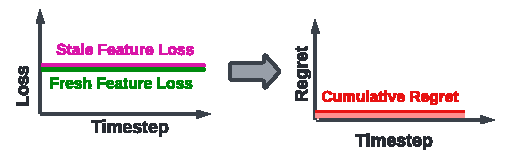
\includegraphics[width=8cm]{ralf/figures/regret_2.pdf}
%    \setlength{\abovecaptionskip}{-2pt}
%    \caption{Constant loss with staleness.}
%    \label{f:regret2}
% \end{subfigure}
% \setlength{\abovecaptionskip}{-0pt}
% \setlength{\belowcaptionskip}{-10pt}
% \caption{Examples of how the prediction loss of the ideal features (green) and the loss of the approximated/stale features (purple) might compare and corresponding regret. 
% %In (a.), increasingly staleness (assuming the feature was updated at t=0) degrades model prediction, and leads to rapidly increasing cumulative regret. In (b.) staleness does not affect the quality of the predictions. Regret still accumulates, but more slowly.
% }
% \label{f:cumulative-regret}
% \end{figure}

\subsection{Feature Store Regret}
\label{ss:regret}
% Approximating feature values to reduce compute resource costs poses the risk of degrading prediction quality of downstream models querying the features. We derive a metric to evaluate the approximation quality of features in terms of downstream prediction accuracy. 

% \subsubsection{Prediction Loss}
% We consider feature tables used in the context of online prediction serving, where models need to query feature values with low latency to process prediction requests. 
% Given a sequence of prediction request data $\{x_{kt}\}$ over keys $k$ and timestamps $t$, we can denote the sequence of predictions generated by the model $m$ in terms of current feature store values $v^t$:
% \begin{equation}
%     \hat{y}(v^t_k) = m\left(x_{kt}, v_k^t\right) 
% \end{equation}
% Each prediction corresponds to some $y$, the true label. The model is trained to minimize the loss $\ell(\hat{y}, y)$ (e.g. mean squared error or top-k error). We can formalize the prediction loss by the serving system as: 
% \begin{equation}
%     \mathcal{L}(m|v^t) = \mathbb{E}_{k\sim Q}\left[\ell\left(\hat{y}(v_t), y\right)\right]
% \end{equation}
% However, we cannot directly use loss to evaluate approximated feature values $\tilde{v}$. First, the true labels may not always be available, preventing observation of the loss. Second, the prediction loss if a function of both the feature values and the model parameters. If a model performs poorly for an out-of-distribution user, the feature store cannot correct the error by improving the quality of that user's features. However if the prediction quality is poor because of out-of-date features, the feature store should attempt to correct this.

%\subsubsection{Feature Store Regret}
We propose a feature store metric, \textit{feature store regret}, to evaluate feature quality. The feature store regret is the difference in predictions made by the optimal feature values $v_k^t$ and approximated features $\tilde{v}_k^t$. 
\begin{equation}
    \mathcal{R}(t) = \mathcal{L}(m|\tilde{v}^t) - \mathcal{L}(m|v^t)
\end{equation}
where $\mathcal{L}(m|\tilde{v}^t)$ and $\mathcal{L}(m|v^t)$ are the \textit{total loss} of predictions made with the approximated and unapproximated feature values, respectively. For simplicity, we assume $\mathcal{L}(m|\tilde{v}^t) \ge \mathcal{L}(m|v^t)$. We can write the total loss in terms of the sequence of prediction requests with data $\{x_i\}$ at time $t$ which correspond to predictions $\hat{y}_i(v_t)$ and true values $y_i$: 
\begin{equation}
     \mathcal{L}(m|v^t) = \sum_{i}\ell\left(\hat{y}_i(v_t), y_i\right)
\end{equation}
where $\ell$ is the loss function used to evaluate the model. 


\subsection{Scheduling with Error Feedback: Regret-Proportional Scheduling}
\label{ss:online-scheduling-error-feedback}
We propose an online scheduling policy in cases where we can observe regret online, which we refer to as \textit{Regret-Proportional} update scheduling. In many model serving applications, the true prediction label can eventually be observed. For example, a recommendation model can serve recommendations to a user and eventually observe which recommendations the user did or did not click through. Similarly, a time series \amit{model can have its predictions evaluated against future observed points}feature can be evaluated against future points observed for the time-series. The observations of the true label can be used to compute model prediction error, which can be used to provide feedback on feature quality. While prediction error cannot always be computed online, we constrain the problem to this setting to consider how error feedback can be used to make better scheduling decisions. 

We formalize the online scheduling problem for feature stores in terms of minimizing feature store regret under resource cost constraints.  At a high level, our proposed policy is to prioritize keys with the highest cumulative regret. 
%This allows us to prioritize updating keys where feature staleness has the highest impact on the overall loss (such as in \cref{f:regret1}) rather than keys where the prediction loss is primarily a result of model error (such as \cref{f:regret2}). 
This allows us to prioritize updating keys where feature staleness has the highest impact on the overall loss rather than keys where the prediction loss is primarily a result of model error. 
We describe how we estimate regret with error feedback in \cref{ss:scheduling-policy}. 
%Assuming the stale version of the feature is always available to be queried, we determine what keys to process updates for.

\subsubsection{Formulation}
We consider a feature table with keys $k\in K$ each mapping to values $\tilde{v}_k^t$. At time $t$, the scheduler can update a subset of keys $U_t \subseteq K$. For each $k\in U_t$, we recompute the feature value on all data up to the current timestamp, while other feature values remain the same. We can denote the approximate feature values at time $t$ with \cref{eqn:delayedupdate} where the staleness $\delta_{k,t}=0$ if the key $k$ is updated at time $t$, and otherwise $\delta_{k,t}=1+\delta_{k,t-1}$. 

Given a constraint $C$ on the number of keys which can be updated at each timestep $t$, our goal is to select updates $U$ such that the staleness matrix $\delta$ minimizes the cumulative regret over time: 
\begin{align}
     \argmin_\delta \sum_t \mathcal{R}(t) \\
     |U_t| \le C, \forall{t}
\end{align}
\subsubsection{Error Feedback}
We assume that we can observe the per-key loss. Say that for the sequence of queries $\{x_{kt}\}$, we eventually recieve error feedback $E_t = \{e_k\}$ denoting the prediction error of $m(x_{kt}, \tilde{v}_k^t)$. For simplicity, we assume that the error is received before we need to make scheduling decisions for the next timestep. We can estimate the per-key loss at each timestep as the sum $\mathcal{L}(m|\tilde{v}_t^ k) \approx \sum_{e_k \in E_t} e_k$.
\sarah{Maybe formalize t?}

\subsubsection{Scheduling Policy}
\label{ss:scheduling-policy}
We propose an online algorithm which selects keys to update based off the cumulative regret observed since the last update: 
\begin{equation}
   \argmax_k \sum_{s=0}^{\delta_{t,k}} \mathcal{R}_k(t-s) 
   \label{eq:cumulative_regret}
\end{equation}
\sarah{Define E TU}

%\subsubsection{Estimating Regret with Feedback}
To estimate $R(t)$, we also need an estimate of the loss with the ideal features $\mathcal{L}(m|v_t^ k)$. We assume that the \textit{expectation} of error over queries is temporally stable with respect to staleness for each key. Thus we can calculate the average error immediately after the feature was updated at time $t_u = t-\delta_{t,k}$ and multiply with the number of error observations at time $t$ to estimate $\mathcal{L}(m|v^t_k)$ and subtract this from each error value observed at timestamp $t$ before taking the sum of all errors observed at $t$. We can thus write out the estimated regret at $t$ as:
% , so we can approximate the unapproximated feature loss as a the loss observed right after the feature was updated (that is, at time $t-\delta_{t,k}$): 
% \begin{equation}
%     \mathcal{L}(m|v_t^ k) \approx |E_{t}|\cdot  \sum_{e_k \in E_{t-\delta_{t,k}}} \frac{e_k}{|E_{t-\delta_{t,k}}|} 
% \end{equation}
\begin{equation}
    \mathcal{R}_k(t) \approx \sum_{e_k \in E_{t}}  e_k -   \sum_{e_k \in E_{t_u}} \frac{ |E_{t}|\cdot e_k}{|E_{t_u}|}  
\end{equation}
Intuitively, we can think of this as computing how much additional error per query there is in $E_t$ (the current timestep error) as compared to $E_{t_u}$ (the post-update timestep error). Expanding out \cref{eq:cumulative_regret} and denoting the last update time as $t_u = t-\delta_{t,k}$, we select the key to update as:  
\begin{equation}
   \argmax_k \sum_{s=0}^{\delta_{t,k}} 
  \sum_{e_k \in E_{t-s}} \left( e_k -   \sum_{e_k \in E_{t_u}} \frac{ e_k}{|E_{t_u}|}  \right)
\end{equation}


%\subsubsection{No starvation} 
We can prevent starvation by upper bounding the regret $R_k(t) < \mathcal{R}_{max}$, and assuming $R_k(t) > \epsilon$ for some $\epsilon > 0$. We find in practice, since the errors in $E_{t_u}$ are relatively small, we can remove the second summation term and simply sum $e_k$ to estimate regret.

\subsubsection{Default Regret}
\label{ss:default-regret}
One potential issue with relying on cumulative regret for key prioritization is that a key may become arbitrarily stale if the key is never queried. Stale keys can be prioritized more by setting a higher minimum regret value $R_k(t) > \epsilon$, so that keys will incur regret over time.



%%%%%%%%%%%%%%%%%%%%%%%%%%%%%%%%%%%%%%%%%%%%%%%%%%%%%%%%%%%%%%%%%%%%%%%%%%%%
% DESIGN
%%%%%%%%%%%%%%%%%%%%%%%%%%%%%%%%%%%%%%%%%%%%%%%%%%%%%%%%%%%%%%%%%%%%%%%%%%%%
\section{System Design and Architecture}
In this section, we describe \system{}, which orchestrates updates to feature tables with adaptation to feedback. Downstream clients query the feature tables through the \system{} client so that \system{} can track query access patterns and also post feedback to \system{} once prediction labels are observed. \amit{Downstream clients query the feature tables through and post feedback to the \system{} client so that \system{} can track query access patterns and the quality of its output}
\sarah{more intuition on the idea of staleness vs. regret?}

% \begin{figure}[t]
% \centering
% 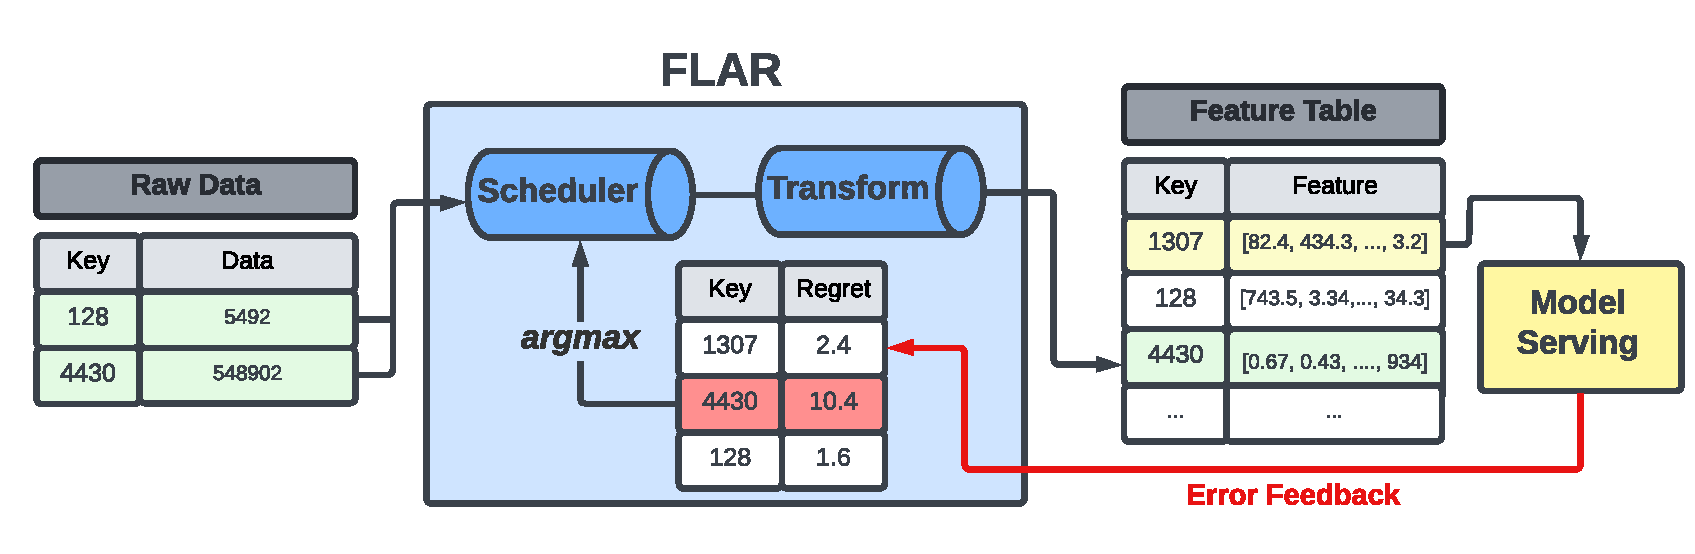
\includegraphics[width=8cm]{ralf/figures/architecture1.pdf}
%  \caption{Overview of a single shard of \system{} Server.}

%  \kevin{Typo in the text above blue box: FLAR -> RALF}
% \label{f:architecture}
% \end{figure}




\label{s:design}
\natacha{It'd be nice to have an overview of what you're going to talk about and even an architecture design "intro". At this point, I'm still unsure what \system{} is}



\natacha{What's the link between shared computation and what we were talking above. Is this a new design? Is is standard feature store architecture??}

\begin{figure}[t]
    \begin{lstlisting}[
language=Python, 
caption=Defining a maintained feature table of user embeddings with RALF. , 
escapechar={|},  
basicstyle=\small,
commentstyle=\color{blue}\sffamily,
stringstyle=\color{red}\sffamily,
numberstyle=\color{gray}\sffamily,
label={lst:api}
]
# Source table 
source = ralf.tables.kafka_source(topic="user_data")

# Queryable feature table 
embedding = source
    .map(UserEmbeddingModel, model_file="model.pt")
    .as_queryable("user_features")
    .set_replicas(4)
    .set_default_error(0.01)
\end{lstlisting}

 
    \begin{lstlisting}[
language=Python, 
caption=Example of a downstream application serving predictions using queried feature values and posting error feedback once the result is observed. , 
escapechar={|},  
basicstyle=\small,
commentstyle=\color{blue}\sffamily,
stringstyle=\color{red}\sffamily,
numberstyle=\color{gray}\sffamily,
label={lst:model_scheduler}
]
class CartAbandonmentModel:
    client = ralf.client(table="user_features")
    cache = {}

    # serve prediction requests 
    def predict(user_id, cart_id): 
        feature, fid = client.get(user_id)
        cache[cart_id] = {
          "pred": model.predict(feature, cart_id),
          "feature_id": fid, 
          "feature_key": user_id
        }
        return cache[cart_id]
        
    # post feedback when label is received 
    def on_label(cart_id, checkout: bool):
        error = MSE(cache[cart_id]["pred"], checkout)
        client.feedback(
          key=cache[cart_id]["feature_key"],
          feature_id=cache[cart_id]["feature_id"],
          error=error
        )
\end{lstlisting}
\end{figure}

% TODO: fix this later
%\RestyleAlgo{ruled}
%\begin{algorithm}[t]
%\caption{Choosing next key to update}\label{alg:choose_key}
%\KwData{List of feedback $F[k]$ for key $k$, $pendingKeys$, $processingKeys$}
%\KwResult{Selected key $k$ to process updates for next.}
%$chosenKey \gets -1$\;
%$maxRegret \gets -1$\;
%\For{$k \in pendingKeys$}{
%$regret = F[k].sum()$\Comment*[r]{Calculate regret}
%
%\If{$regret \ge maxRegret$}{
%$maxRegret\gets regret$\;
%
%$chosenKey\gets k$\Comment*[r]{Update chosen key}
%}
%}
%$F[chosenKey] = []$\Comment*[r]{Clear key feedback}
%$pendingKeys.remove(key)$\;
%$processingKeys.append(key)$\Comment*[r]{Key is processing}
%\Return chosenKey
%\end{algorithm}

%
%\subsection{Operators for Featurization}
%\label{ss:design:operators}
%
\subsection{\system{} Server}
\natacha{What you're describing here doesn't seem to be an an API, but a design?}
\system{} orchestrates data updates to maintain feature values. We show an example of defining a maintained feature table with \system{} in Listing \ref{lst:api}. 
%We show a high-level overview of \system{} in \cref{f:architecture}. 
\system{} schedules and processes data updates to compute new values for the feature table using the specified feature transformation. In addition, \system{} receives queries and error feedback from the client in order to track feature access patterns and quality. \system{} requires a feedback loop: a downstream model that queries feature values must post the observed error for the corresponding key back to the server. This data is used by the scheduler to help decide which key to update next.


\subsubsection{Transformation}
Feature transformations are defined by user definted functions (UDFs) which can maintain state and define an \textit{on\_event} function, which define how to transform a data update from the raw data table to a data update to the feature table. We show an example transformation in Listing \ref{lst:api}. These transformations are implemented as Ray actors, so \system{} relies on Ray for concurrency and fault tolerance.

\subsubsection{Scheduling}
Pending updates are scheduled by \system{} with the scheduler, which chooses the next key to update. The scheduler receives error feedback from downstream models, and uses this to update a table tracking estimated cumulative regret per key. This table is used to select the key with the highest estimated regret. 
The chosen key and corresponding data passed to the transformation.

\subsubsection{Scaling}
\system{} scales to large cardinality datasets by sharding keys across multiple replicas, which each replica can run on separate processing across a single or multiple machines. Each replica has a separate scheduler and error table to avoid coordination.  


%Similar to existing streaming systems, \system{} defines a computation pipeline as a DAG of operators over an incoming stream of data. The output from the computation pipeline represents updates to some materialized feature view, for which we accumulate feature store regret. Each operator in \system{} has scheduling queue for updates, which selects keys with maximal regret. \system{} additionally provides a simple API for downstream applications to query features and post error observations, so that \system{} can allocate feature updates to better optimize for downstream accuracy. 


%\system{}'s API defines featurization pipelines in terms of a DAG of \textit{feature tables}, where each feature table is defined in terms of terms of an operator and one or more input (i.e. parent) feature tables. Feature tables can be make externally queryable through an HTTP interface, and are incrementally updated as new data is streamed into the pipeline. We show an example definition of a feature table in Listing \cref{lst:api}.
%Similar to streaming dataflow systems, \system{} consists of a set of operators chained into a DAG.
%
%
% For example, a featurization pipeline which detects anomalies across a rapidly-changing time series
% (\cref{ss:evaluation:time-series-decomposition}) benefits more
% from a smaller window slide size compared to a stable time series.
% \peter{Consider adding a small experiment to elaborate on/quantify this}
% \sarah{Maybe we could improve figure 2 and reference it here, since it's showing how some time series in the yahoo dataset need very few re-fits}
% %
% The smaller slide size generates more frequent updates, which enables the rapid detection of anomalous changes
% in the time series by downstream operators.
% %
% On the other hand, generating more updates results in more work for downstream operators which may
% run expensive anomaly detection models.
% %
% Because time series for different keys may change at different rates, \system{}'s window operator will
% re-configure each key's window configuration in order to find the ideal trade-off between cost
% and delay in anomaly detection by optimizing the latency-aware feature store accuracy.
% \natacha{This paragraph feels a little strange as it sounds like you didn't have Section 3, and you don't talk about Section 3 at all here. Presumably, isn't the reason why you support per-key window configuration a response to the "findings" you made in Section 3? }
%
% Thus, dynamically adjusting per-key window slide size at runtime can balance compute costs for
% timely anomaly detection by optimizing the latency-aware feature store accuracy.
%

%

%

%\system{} innovates on both the window operator and map operator. 

% \myparagraph{Window Operators}  While traditional windowing operator only allow setting a fixed sized window for the entire stream, \system{}'s windowing operator allow per-key window configuration. For example, in the anomaly detection model use case \kevin{explain earlier what this is}, a time series that's rapidly changing would benefit more from smaller sliding size for a sliding window operator as compare to a very stable time series. For rapidly changing time series, maybe we should emits the sliding window every 2 records to capture any recent changes; while for a stable time series, we can just emits a sliding window every 128 records \kevin{is this very application specific?}. The smaller the slide size, the more records that the downstream operators need to process, therefore increase the compute cost; but smaller the slide size also means we will be capture the freshest data in downstream operators and drive up accuracy. Therefore, *per-key window configuration* allows \system{} to balance compute cost and feature accuracy intelligently. This feature can be implemented as custom windowing operator in traditional streaming dataflow system, however \system{} made it built in and as a first class primitive.
% \sarah{this per-key thing applies to all operator scheduling parameters though, right?}

\subsection{\system{} Client}
The \system{} client is used by downstream applications to query \system{} for features and to post feedback. We show an example of a downstream application in Listing \ref{lst:model_scheduler}, which queries the client for feature values to predict the likelihood of cart abandonment. For applications where true labels are later provided, the application can also post feedback to the client to inform future scheduling the decisions. The feedback takes in the key of queries feature, the queried feature version, and the error of the resulting prediction. Feedback is posted to \system{}, which tracks error feedback for current feature versions on the feature view.  

\subsection{Scheduling Policy}
\label{ss:design:scheduler}
%
\system{} schedules feature updates with Regret-Proportional scheduling, that is, prioritizing updates to keys with the largest \textit{cumulative regret}. The cumulative regret is calculated by tracking the reported error for predictions made using the current feature version stored in the table, and then selecting the key with the largest cumulative regret (as shown in Algorithm \ref{alg:choose_key}). Once a key is chosen, the prior feedback and queue for the key are both cleared, and the key is marked as being processed and locked until the new feature value is computed. The scheduler tracks a list of \textit{pendingKeys}, the list of keys with new data updates, and \textit{processingKeys}, the list of keys where new features are currently being computed. Keys are selected from \textit{pendingKeys}, and once selected, are removed from \textit{pendingKeys} and added to \textit{processingKeys}. Keys in \textit{processingKeys} cannot be chosen again by the scheduler until they are removed once the featurization update is complete - this is to prevent duplicate updates to keys while they are still processing. 


\subsection{Implementation}
\label{ss:design:implementation}
%
\jmh{It's a missed opportunity not to do this in a DBMS with UDFs like Postgres, and talk about materialized views. If you had done so, you'd have a very VLDB-friendly exposition of the APIs, clean example code, clear view materialization opportunities, etc.}
%
%
We construct a full prototype of \system{} in about 1,500 lines of Python code.
%
Our prototype is built atop Ray~\cite{ray}, because many
popular featurization and machine learning libraries (e.g., Tensorflow~\cite{tensorflow})
use Python, and Ray is designed to support machine learning workloads.
%
We emphasize that \system{} is a set of ideas for accuracy-aware featurization, and
can be implemented on several systems. 
% In particular, \system{} can also be implemented as an algorithm to optimize materialized view maintenance in traditional relational database. We chose 

% To show the generality of our contributions, we also provide a reference implementation
% in Timely Dataflow~\cite{timely-dataflow-book}.
%
%
%\myparagraph{Ray prototype}
%

%\jmh{To me the only value of the multiple implementations is to convince the skeptical systems reader that you've solved the problem in a portable way. See my comment below in related work. I wouldn't dwell on evaluating Ray vs Timely vs Noria. Phooey. Now, if one of them lacks the expressivity you need to do the right thing, DO bring that up here, but don't run an evaluation to establish an expressivity problem. By contrast, if one of them is more efficient---e.g., provides a faster update rate---is that really pertinent to your contribution of reframing the feature store freshness problem? Or is it just kind of "System X is more efficient at the class of queries you see here than System Y", but it's not fundamental -- these queries could be tuned up in System Y orthogonal to our techniques. I care more about you characterizing that class -- and then letting the systems optimize for it later if they choose. Finally, there are many systems here you're not evaluating that can express this stuff---notably many database engines---which makes this feel to me like pandering to a narrow audience and its myopia. In the real world I might want to use Snowflake or a high-performance main-memory database; I'm probably not gonna use Noria or Timely. Independent of these pragmatics, why does this paper care anyhow? I feel like you're soiling your beautiful big idea of ``it's the application metric that matters, stupid''  with other people's obsession with system internals of research prototypes. (Grumpy database guy signing off!)}

% \system{} is a set of ideas that bring ML feature quality awareness into streaming dataflow system. It it agnostic to any underlying systems. For this paper, we implemented a prototype system on Ray and a comparison system on Timely Dataflow. We chose to implemented on Ray because it's easy to integrate Python based featurization pipeline and machine learning libraries into the streaming pipeline.
% 
% For the Ray prototype implementation, each operator runs on Ray Actors. Each operator can be sharded by record key. Sharding makes it easy to horizontally scale out the processing throughput. We then use Ray's actor call as RPC mechanism to send records among the operators. 
%
% For the timely dataflow implementation,

% \myparagraph{Offline planner}
% The offline planner was built using an off-the-shelf discreate event simulation library, simpy \cite{matloff2008introduction}. We use the simulation library to generate traces with samples of production workload and compute its accuracy score. To optimize the featurization policies across keys, we use a mixed integer linear program solver (OR-tools \cite{van2014or}) to optimize the final feature policies. The linear program is written to solve for the lowest cost combination of feature policy per key, under a compute budget constraint.


%%%%%%%%%%%%%%%%%%%%%%%%%%%%%%%%%%%%%%%%%%%%%%%%%%%%%%%%%%%%%%%%%%%%%%%%%%%%
% EVALUATION
%%%%%%%%%%%%%%%%%%%%%%%%%%%%%%%%%%%%%%%%%%%%%%%%%%%%%%%%%%%%%%%%%%%%%%%%%%%%
\section{Evaluation}
\label{s:evaluation}
% table of workload characteristics
\begin{table*}
\centering
\label{table:workloads}
\caption{Workload attributes. The \textit{Runtime} column refers to the featurization update runtime for a single key. The \textit{Min Loss} and \textit{Max Loss} columns show the overall loss given infinite budget and zero budget for featurization, respectively. The minimum loss for the Azure dataset is shown in \cref{f:stl-time}. }
\begin{tabular}{|l|l|l|l|l|l|l|l}
\cline{1-7}
\textbf{Workload} & \textbf{Dataset} & \textbf{Keys} & \textbf{Runtime} & \textbf{Edits}  & \textbf{Min Loss} & \textbf{Max Loss} &\\ \cline{1-7}
Recommendation & MovieLens 1M & 6041 & 0.9s & 85,297 & 1.12 & 6.29 & \\ \cline{1-7}
%IR & Wikipedia Edits & 200 & 1.1s & 16,342 & 75.3\% & 94.3\% &  \\ \cline{1-7}
 & Yahoo Anomaly A1  & 68 & 0.25s & 43,684 & 90.79 & 880.3 & \\ \cline{2-7 }
\multirow{-2}{*}{\begin{tabular}[c]{@{}l@{}}Time-Series \\ Decomposition \end{tabular}}  & Azure VM Dataset  & 275,077 & 0.4 & 5,683,390 & - & - & \\ \cline{1-7}
\end{tabular}
%\vspace{-2em}
\end{table*}

In this section, we address two primary questions: (1) how does Regret-Proportional scheduling impact downstream prediction accuracy (2) how does \system{} with Regret-Proportional scheduling scale to processing high-cardinality, high-rate data streams? To answer these questions, we structure our evaluation as following:
\begin{enumerate}
    \item We construct representative workloads for two common feature store use-cases, recommendation and anomaly detection, using real-world datasets. For both workloads, we evaluate feature quality by evaluating model predictions that rely on feature which are updated over time. 
    \item We run an end-to-end evaluation with \system{} on a large-scale anomaly detection workload to evaluate prediction accuracy improvements, system overhead, and scaleability. 
    \item We run ablations comparing Regret-Proportional scheduling with both baseline and application-specific policies. 
\end{enumerate}



\subsection{Workloads} 
\label{ss:workloads}

%\noindent\textbf{Workload Generation.}
\label{ss:evaluation:workloads}
To evaluate feature maintenance policies, we construct workloads using real-world data where model predictions rely on pre-computed features that need to be updated as new events are streamed in. For each workload, we use real-world data to generate an \textit{update stream} (incoming raw data),  \textit{query stream} (queries from downstream models), and \textit{feedback stream} (error feedback). 

For each workload, we setup to following components to mimic realistic prediction serving applications: A  \textbf{feature function} (the operator that transforms data streams into features cached in the feature table), \textbf{feature table} (the key/value store contained feature keys and values), and \textbf{downstream model} (the downstream prediction serving application which queries feature table values that are used to make predictions). 

We describe the dataset, featurization, and downstream models for recommendation and anomaly detection workloads. A summary of workload attributes is show in \cref{table:workloads}, which also shows the best and worst-case prediction loss depending on feature quality. 


\subsubsection{Anomaly Detection}


Time series decomposition is a common pre-processing step to many downstream tasks, such as anomaly detection or forecasting. We construct an time-series anomaly detection workload based off a real-world application at Splunk \cite{wang2021online,mishra2021onlinestl}. The anomaly detection task compares predicted points from time-series features, calculated from windows of past data, with the observed points to detect anomalies. Accurate anomaly detection depends on estimating the residual of the point accurately, which relies on the accuracy of the cached time-series features. The \textit{query stream} periodically queries all keys to detect anomalies in regular time-intervals, so the distribution of queries over keys is uniform. Features are maintained over an \textit{update stream} of new time-series points. Each new time-series point is compared to previously predicted points to provide a \textit{feedback stream}.

\myparagraph{Dataset}
We use both the Yahoo Webscope S5 Dataset's A1 class \cite{laptev2015yahoo} and Azure VM dataset \cite{cortez2017resource}.\sarah{I could have both teh graphs for yahoo and azure, but they look the same...} We use the Python statsmodels library \cite{seabold2010statsmodels} to compute features from windows of data for each time-series. For the Yahoo dataset, the rate of updates and start time for each time-series is uniform across keys, so the distribution of queries and feedback across keys is also uniform. However, the variation in the time-series can vary dramatically across keys, opening opportunity for optimizing resource allocation across keys. For example, some time-series vary little over time, while others change rapidly and have complex and variable seasonality components. \sarah{add example time-series?}

% new for the revision, more description about the Azure dataset - simon



%\myparagraph{Scheduling Policies} We implement a baseline policy as a round-robin policy (\textit{roundRobin}) which iterates over keys to choose which key to update next. We also implement our scheduler described in \cref{ss:online-scheduling-error-feedback}, which we refer to as the \textit{regret optimized} scheduling policy. Altough the staleness of the queried keys is minimized by the round robin policy, as shown in \cref{fig:stl-yahoo-staleness}, minimizing feature staleness does not necessarily minimize prediction loss. We show the average error across keys in \cref{fig:stl-yahoo-error}, where the regret optimize has significantly lower average prediction loss across queries as compared to round-robin. The regret optimized scheduler is able prioritize keys which are more likely to degrade prediction accuracy using error feedback. We show in \cref{f:stl-a1-heat} the most frequently updated keys by the regret optimized scheduler, and the corresponding number of updates for the same keys by the round robin scheduler. 


\subsubsection{Recommendation}

Recommendation is another applications where machine learning models are used to make low-latency recommendations to users, often using user features derived from historical data to personalize predictions. We construct a recommendation workloads where a downstream models predicts what a user's rating for a movie will be user and movie features computed from past rating data, where user features are updated online. Given a stream of user ratings for movies, we simulate a \textit{query stream} over the users to predict what the rating should be. We return the prediction error of the rating as the \textit{feedback stream}, and treat the rating itself as data update from the \textit{event stream}. The incoming event stream of ratings is used to update user embeddings over time using partial ALS to update the corresponding feature vector. 

\myparagraph{Dataset}
We use the MovieLens 1M \cite{movielens1m}, which has timestamped ratings from roughly a million user/movie pairs. We use the first half of the data to train a model using Alternating Least Squares\sarah{cite?}. We treat the resulting movie embeddings as the static \textit{model} and the user-ratings as \textit{features} which are updated over time. We use the second half of the data as query, event, and feedback streams. 

%\myparagraph{Scheduling Policies} In addition to round robin, we implement two additional natural baseline policies: 1. selecting the key with the maximum pending updates (\textit{maxPending}), 2. selecting the key with the fewest observed data points (\textit{minPast}). We also implement our regret optimize policy using the error feedback from the rating predictions. We find that \textit{minPast} and \textit{regret} perform significantly better than other policies, as they prioritize updating users with the least amount of prior information. For more resource constrained settings, we find that \textit{regret} still performs substantially better than  \textit{minPast}. For keys updated the most frequently by round robin, we show the number of updates allocated by other policies in \cref{f:als-heat}. Due to variation the number of users receiving updates over time, the distribution of updates is similar between policies. However this slight variation in updates is enough to dramatically affect accuracy.




%Time series decomposition is a common pre-processing step to many downstream tasks, such as anomaly detection or forecasting. We construct a time series decomposition featurization pipeline based off real-world workloads at Splunk. Time-series data from many different sources decomposed into trend and seasonality components. These trend and seasonality estimates can be used to evaluate the \textit{residual} (or noise) of later points in the time-series, which can be used for anomaly detection tasks. 

%We evaluate the state of the feature store based off the quality of the \textit{residual estimates} of the downstream task. The downstream anomaly detection task calculates a residual for each new point for each time-series by querying the time series ID from the feature table to obtain the time series' features. We use the loss of the residual estimate to evaluate the features, using the residual calculated from fitting the STL model to the entire dataset as the "ground truth" residual estimate. We generate a query pattern which regularly queries all keys in the feature store to generate residual estimates (for anomaly detection) for all keys. 

 

\subsection{End-to-End Evaluation}
% Full Azure Figure 
\begin{figure*}[t]
\begin{center}
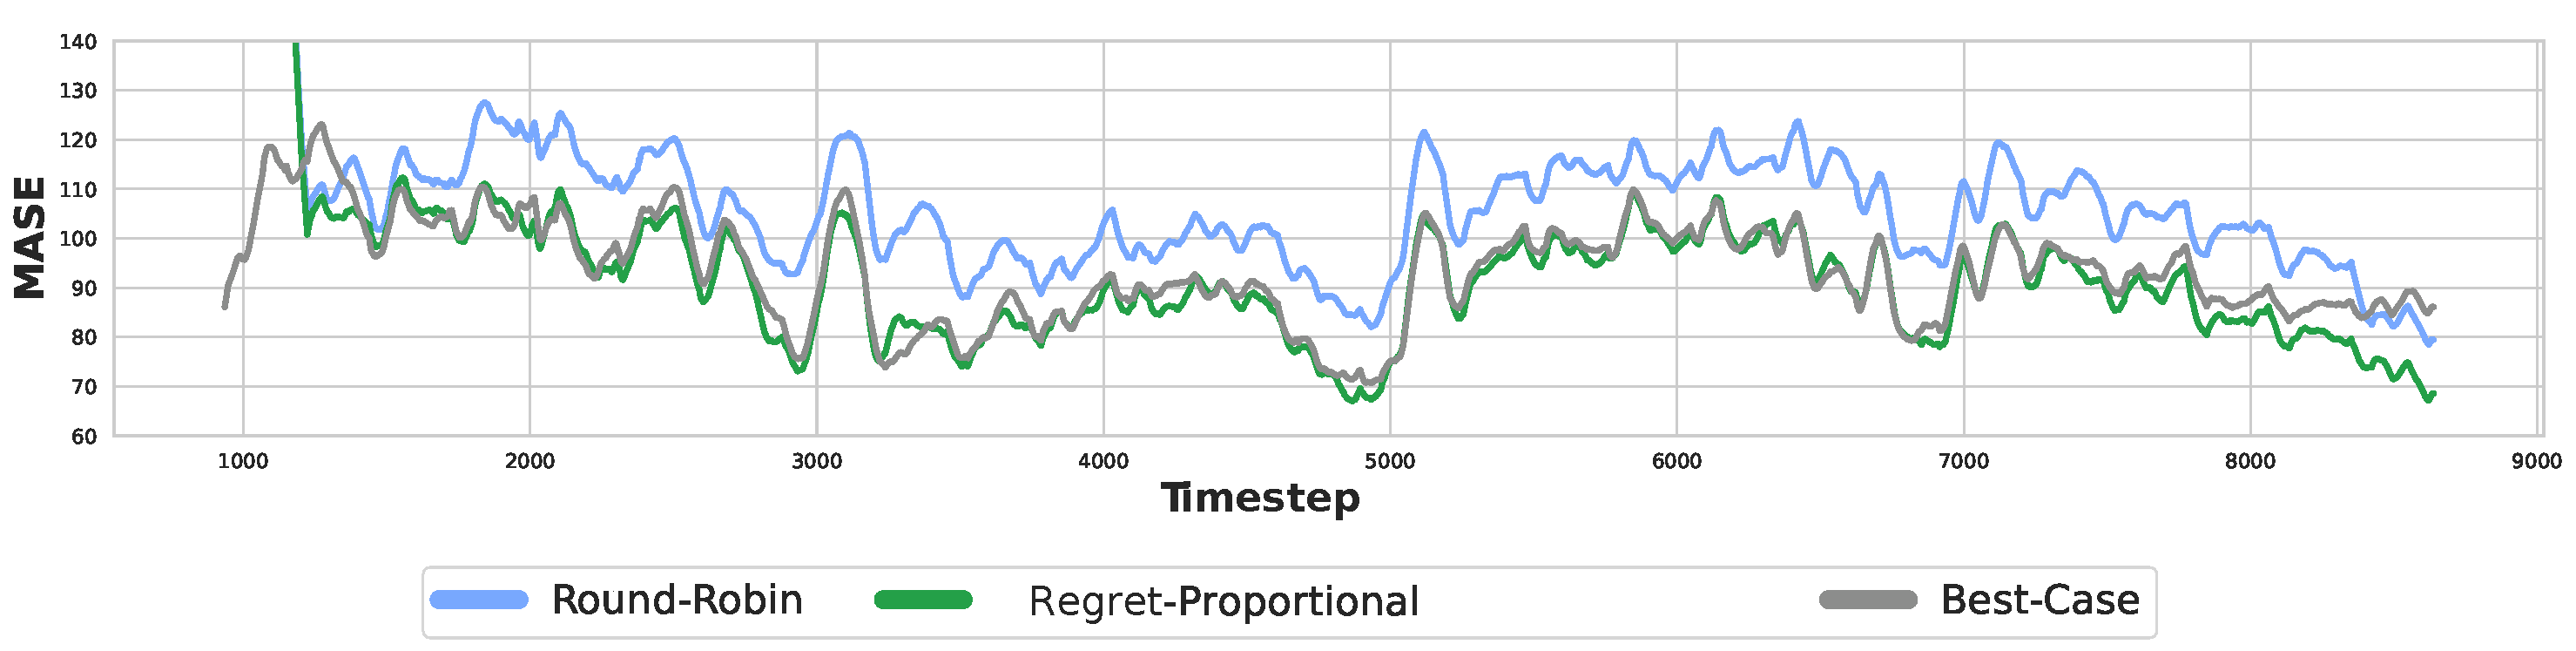
\includegraphics[width=15cm]{ralf/figures/ralf_azure.pdf}
\centering
\end{center}
\caption{Smoothed Average MASE per Timestep over 275,077 keys.
%We calculate MASE across all 275,077 keys at each timestep for the Regret-Proportional, Round-Robin, and Best-Case features. The Regret-Proportional policy closely matches error as if we have infinite resources. Compared to the Round Robin policy, Regret-Proportional policy averages to 13.3\% and peak at 32.7\% error improvement.
}
\label{f:stl-time}
\end{figure*}

We evaluate \system{} on 800 cores for end-to-end with the Anomaly Detection workload using the Azure VM dataset \cite{cortez2017resource}. We run \system{} with both our Regret-Proportional policy and baseline policy of Round-Robin scheduling to evaluate prediction accuracy, scheduling overhead, and scaleability.  

\subsubsection{Experimental Setup}
The Azure VM dataset includes of the CPU readings taken every 5 minutes on a pool of 2 million VMs over the span of one month. We send a subsample of 275,077 time-series from Azure Dataset on a cluster of 11 m5d.24xlarge machines (800 cores) on AWS. We simulate higher data send rates by sending at 1000x speed (i.e. ingesting data once every 0.3 seconds, rather than every 5 minutes as specific in the dataset). We use \system{} to compute an STL decomposition of the time series for each key, using a recent observation window. We set the STL decomposition seasonality to be 24 hours, and set the observation window size of data to be 3X the seasonality length (so 72 hours of recent data points) to have a sufficiently large window to compute the decomposition. We store the resulting STL decomposition as a feature in the feature store for each key (i.e. a time-series ID), which is updated over time by \system{} as new data arrives. Because of the high data rate, some features will be out of date with the current observation window. \system{} uses either the Regret-proportional or Round-Robin scheduling policy to choose which features to prioritize updating.

\subsubsection{Policy Error}
To evaluate feature quality, we compare the MASE (Mean Absolute Squared Error) of time-series predictions using the STL decomposition features using the Regret-Proportional and Round-Robin scheduling policies in \cref{f:stl-time}. We can calculate the MASE by comparing the predicted points with the actual points observed. We show a plot of average MASE across keys over time for features computed with the Regret-Proportional and Round-Robin scheduling policies in \cref{f:stl-time}.  Although overall MASE varies over time, the Regret-Proportional policy consistently produces lower MASE than the Round-Round policy features, with error improvement ranging from 2-32.7\% and averaging to 13\%.

We additionally calculate the \textit{optimal} version of the features (described in \cref{ss:regret}) for each query by calculating what the feature value would be with all data up to exactly the query time. The optimal features correspond to the best case MASE (shown in grey in \cref{f:stl-time}) enabled by unlimited compute resources (i.e. processing every possible update). We see that the MASE for optimal features and the Regret-Proportional policies are similar in \cref{f:stl-time}. The Regret-Proportional policy over the course of the experiment runs 61\% fewer updates (i.e. $1.6\times$ less) than would be needed to achieve the optimal features, however averages only 1\% additional error as compared to optimal features. 

%Infinite resource is simulated because it takes ~2x the resource as compared to both policy. On full scale of the the Azure Dataset, Regret Optimized policy only needs to evalaute 61\% of the windows to match the error (with 1\% penalty) of using evaluating all the windows.

\subsubsection{Scaling Evaluation}
We evaluate how \system{}'s throughput scales in  \cref{f:stl-throughput} by measuring the throughput per number of cores for Round-Robin versus Regret-Proportional scheduling. For both the Round-Robin and Regret-Proportional policies, the throughput scales linearly with the number of cores. Because the workload is embarrassingly parallel, we can shard keys across replicas, where each replica corresponds to one core and has its own scheduling and transformation operator. As a result, the number of updates scales linearly with with the number of cores. We use randomized hashing to place keys on replicas and utilize 800 cores of workers.

\begin{figure}[t]
\begin{center}
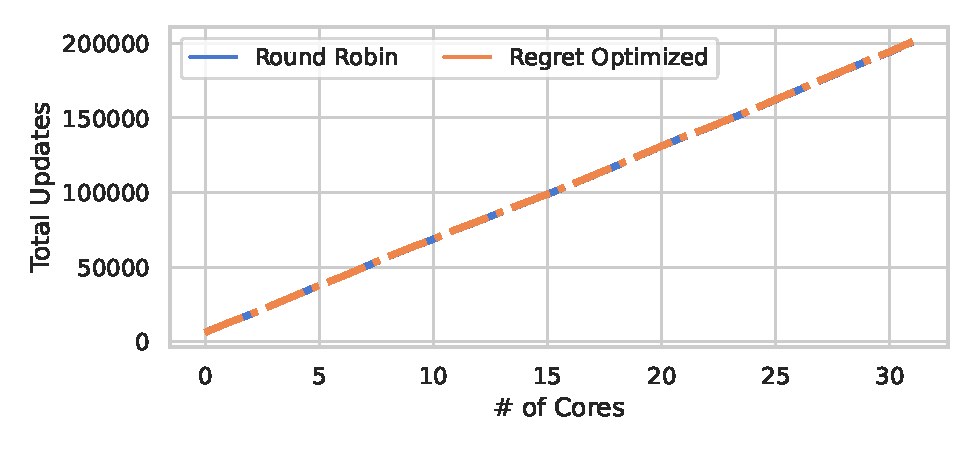
\includegraphics[width=6cm]{ralf/figures/scaling-april-15-10k-keys.pdf}
\centering
\end{center}
\caption{System throughput versus number of cores.}
%\textcolor{red}{TODO: potentially add graph of time in scheduling, workload breakdown, number of updates difference. Add memory size? Throughput per core?}
\label{f:stl-throughput}
\end{figure}

\subsubsection{Scheduling Overhead}
\label{s:overhead}
%We observe about a $1\%$ overhead with Regret-Proportional scheduling compared to Round-Robin, however this overhead is constant with respect to the number of cores, as shown in \cref{f:stl-throughput}. 

We evaluate the scheduling overhead of Regret-Proportional versus standard Round-Robin scheduling in terms of both compute and memory. The Regret-Proportional policy requires  a constant CPU cost of 300 $\mu s$ per arrived window queued for update in order to evaluate the regret score. Furthermore, maintaining a sorted queue (ordered by per-key regret) costs 50 $\mu s$ per addition/removal. Additionally, because the regret calculation requires previous feature to be cached in memory, the Regret-Proportional policy also costs about 32 KBs per key, resulting in about 11MB of memory overhead per core. We note that the per-core compute and memory overhead is constant regardless of the number of cores used, due to scheduling occurring per-replica rather than globally. This allows us to mitigate coordination overhead and is sufficient for making scheduling decisions that load balance across threads and optimize feature quality. 

%The overhead is fairly small and does not increase with scaling as \system{}'s scheduler is run each individual worker instead of using a global scheduler. 

%With large enough keys to prioritize within the worker, the localized scheduling decisions closely resemble those of a global scheduler. For example, in the previous scaling experiment on 800 cores, each worker gets to schedule the computation over ~350 keys. 

We plot the total throughput as a function of total cores in \cref{f:stl-throughput}. The Regret-Proportional policy performed 0.6\% less updates as compared to Round-Robin policy. However, despite fewer number of updates performed, the cached features from Regret-Proportional scheduling results in significantly better model performance. This is because the Regret-Proportional policy can achieve similar feature quality with dramatically fewer updates, as shown by achieving near-optimal feature quality with 61\% fewer updates.




\begin{figure*}[t]
     \centering
    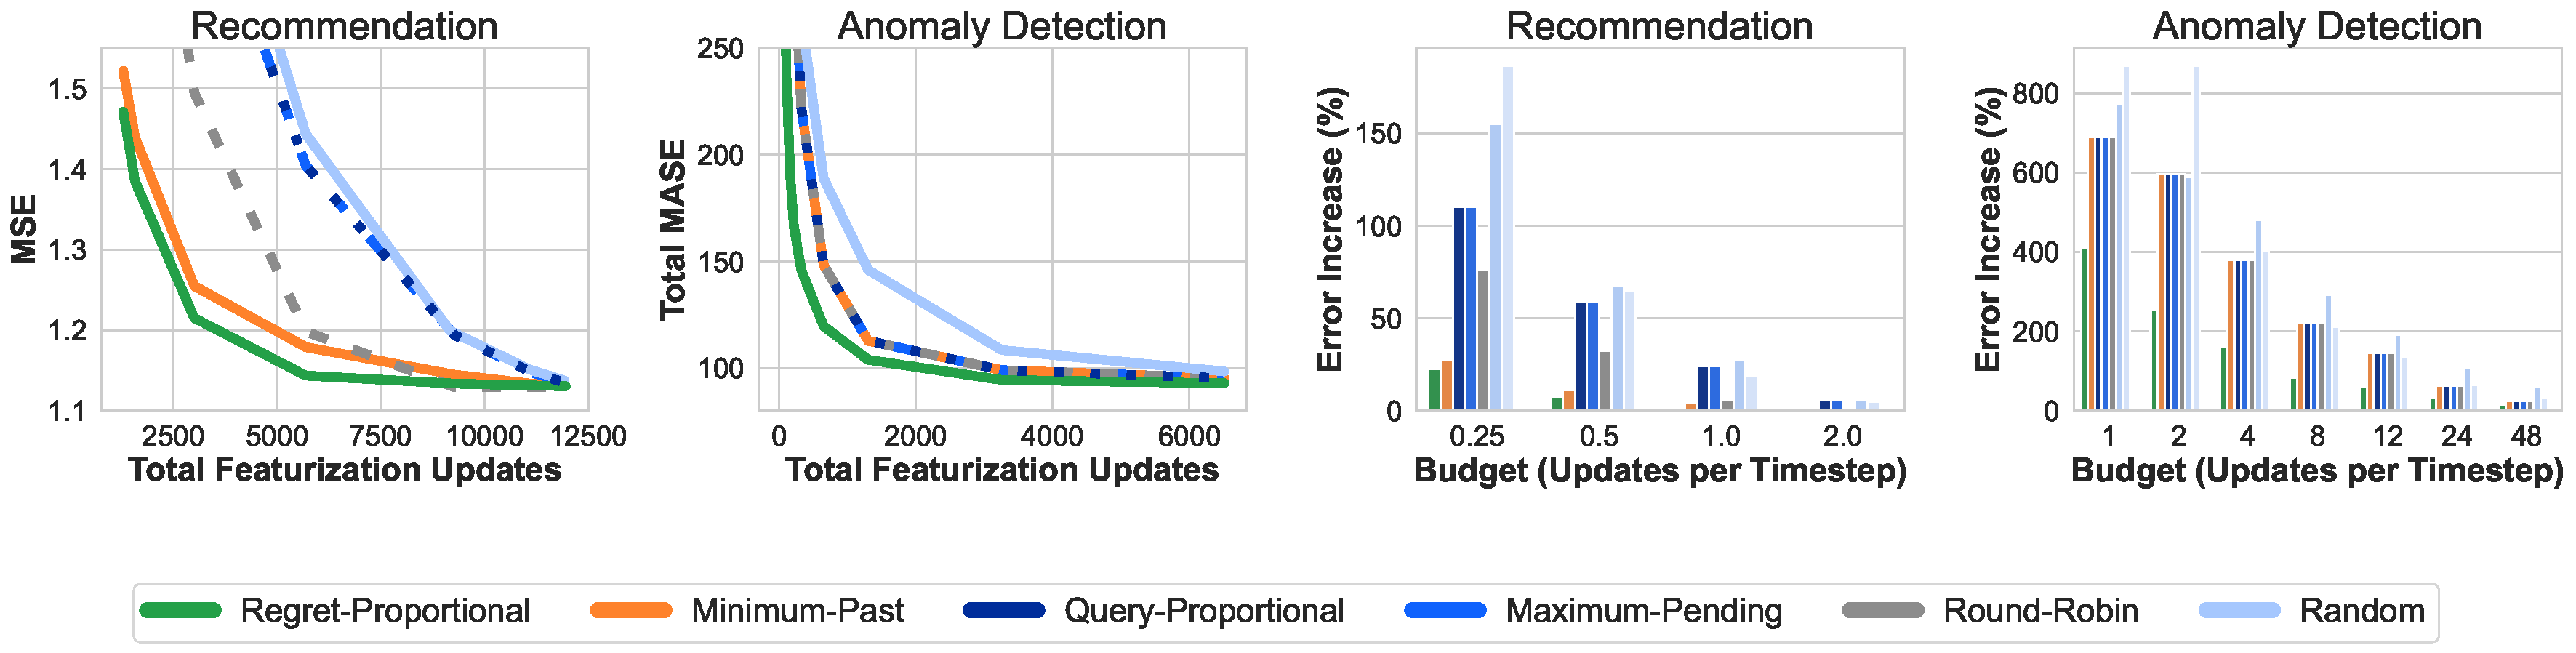
\includegraphics[width=17cm]{ralf/figures/line_all_no_ir.pdf}
    \caption{Left: Prediction error versus total featurization updates (over the entire experiment). Right: Error increase (compared to optimal features with unlimited budget) for varied update budgets.}
    \label{fig:results-all-line} 
\end{figure*}

\subsection{Policy Ablations}
We compare the Regret-Proportional scheduling policy to other baseline and application-specific policies that do not consider downstream prediction accuracy. We run simulated experiments with both the Recommendation workload and the Anomaly Detection workload (using a smaller time-series dataset, the Yahoo A1 dataset) to show the generality of our policy improvements.  
\label{s:policy-evaluation}


\subsubsection{Policies}
We implement the \textbf{Regret-Proportional} policy described in \cref{ss:online-scheduling-error-feedback}. Similarly, we implement a \textbf{Query-Proportional} policy which updates features proportionally to the rate they are queried (i.e. the number of times the feature has been queried since last updated), to understand the impact of regret versus query awareness.  We evaluate these policies along with baseline query-oblivious policies commonly found in stream processing systems. 


We implement baseline query-oblivious policies for choosing which keys to update: 
\begin{itemize}
    \item \textbf{Round-Robin}: Iterate over each key and skip keys with no pending updates (equivalent to updating the most stale and least-recently-updated key). 
    \item \textbf{Random}: Randomly select a key with pending updates. 
\end{itemize}
We additionally implement two more sophisticated query-oblivious policies designed to improve accuracy in the Recommendation workload:  
\begin{itemize}
    \item \textbf{Minimum-Past}: Update keys that have the least data incorporated into the feature (i.e. the number of ratings seen for the user). 
    \item \textbf{Max-Pending}: Update keys with the most pending new data (i.e. the user with the most new ratings).
\end{itemize}



\subsubsection{Prediction Error }

To evaluate the quality of features derived with different policies under different cost constraints, we simulate the policies for each workload.  
%
At each timestep in the simulation, there is a set of feature update events and feature queries for a set of prediction at that timestep. 
%
We set an update budget, which limits the number features we can update per timestep. 
%
The subset of features to update is chosen by the scheduling policy. 
%
At each timestep, the simulator processes some subset of feature updates chosen by the scheduler and generates predictions using the current set of features, which we use to evaluate error in \cref{fig:results-all-line}. 

%The features are used to evaluate the overall prediction error incurred over time, which we use to compare the results of different policies.
%
\subsubsection{Regret-Proportional Policy}
The Regret-Proportional policy is able to achieve better error across different workloads and numbers of udpates, as shown in \cref{fig:results-all-line}. Query-Proportional updates improves error over baseline policies for the Anomaly Detection workload, as shown in Figure \cref{fig:results-all-line}. However for the Recommendation workload, where it is crucial to update features with little prior data (e.g. new users), the updating proportionally for the queries fails to account for the non-uniform benefit of updates across features. As a result, the Minimum-Past policy, which updates the feature with the fewest prior updates, significantly outperforms the Query-Proportional policy for Recommendation. Weighing the queries by the regret they incur (as in the Regret-Proportional policy) improves the results beyond Query-Proportional updates alone by accounting for \textit{both} the query pattern and the significance of updates. 

%\subsubsection{Minimum-Past vs. Regret Proportional}
New users who have no associated ratings (and hence very poor quality default features) are prioritized by Minimum-Past and Regret-Proportional policies, which significantly improves performance over other policies. However, Minimum-Past cannot distinguish the important of updates between users with similar prior update histories, resulting in worse performance than Regret-Proportional overall. We measure the MSE improvement from the Regret-Proportional policy over Minimum-Past for users with past ratings (Trained) versus new users (Untrained) in \cref{f:user_variance}. Although both policies are similar for new users, the Regret-Proportional policy has substantial improvements over Minimum-Past for existing users keys. The Regret-Proportional policy is able to account for the importance of prioritizing updating new users' features, while also intelligently prioritizing updates across users for which features have already been computed. 


\begin{figure}[t]
\begin{center}
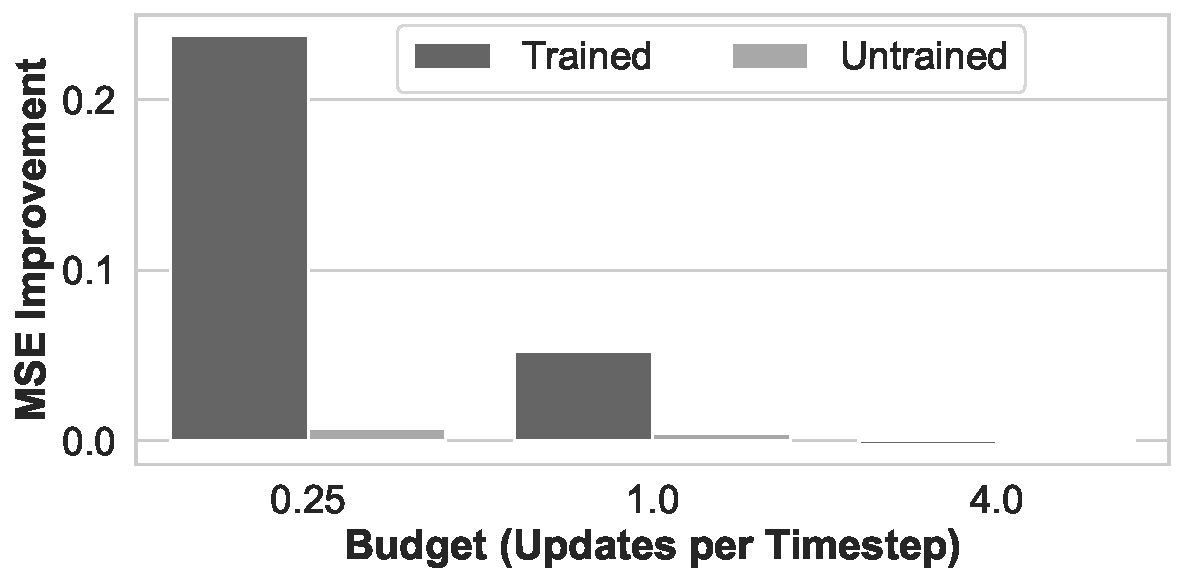
\includegraphics[width=6.5cm]{ralf/figures/user.pdf}
\centering
\end{center}
\caption{Regret-Proportional Improvement over Minimum-Past for users in the training set (Trained) versus new users (Untrained) in the Recommendation workload. }
\label{f:user_variance}
\end{figure}


\subsubsection{Distribution of Updates}
Different policies allocate update budgets in different ways across keys. The variation is most clearly observed for the Anomaly Detection workload, where keys have raw data updates and queries arriving at uniform rates, but are updated with very different distributions depending on the policy, as show in \cref{fig:stl-yahoo-staleness}. The Regret-Proportional policy is able allocate more updates to features incurring regret the most rapidly, resulting in large update variations.


\begin{figure}[t]
\begin{center}
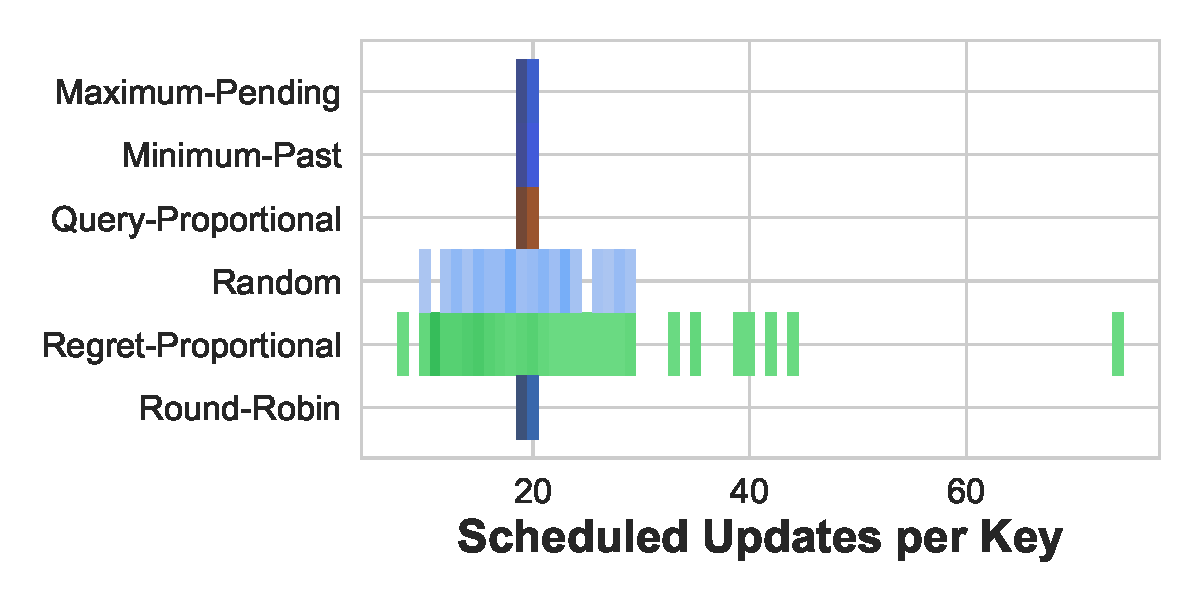
\includegraphics[width=7cm]{ralf/figures/azure_updates_hist_tmp.pdf}
\centering
\end{center}
\caption{\textbf{Distribution of featurization updates (Anomaly Detection):} The Regret-Proportional policy has the most variability in number of updates per key.}
\label{f:update_variance}
\end{figure}

\subsubsection{Optimizing Feature Staleness versus Feature Quality}
Although the staleness of the features is correlated to the prediction accuracy as shown in \cref{f:staleness}, we find that the best performing policies in terms of prediction error are not the best performing in terms of staleness data. As shown in \cref{fig:stl-yahoo-staleness}, the Regret-Proportional has higher average staleness than other policies, including Round-Robin. This is because other policies such as Round-Robin will always prioritize updating the most stale feature, rather than the most important feature to update to optimize downstream prediction error. 
As a result, the Regret-Proportional policy results in better prediction error despite increased staleness, as shown in \cref{fig:results-all-line}. Although staleness is strongly correlated to feature quality, optimizing for staleness does not always have the same results as directly optimizing for feature quality. 

\begin{figure}
    \centering
    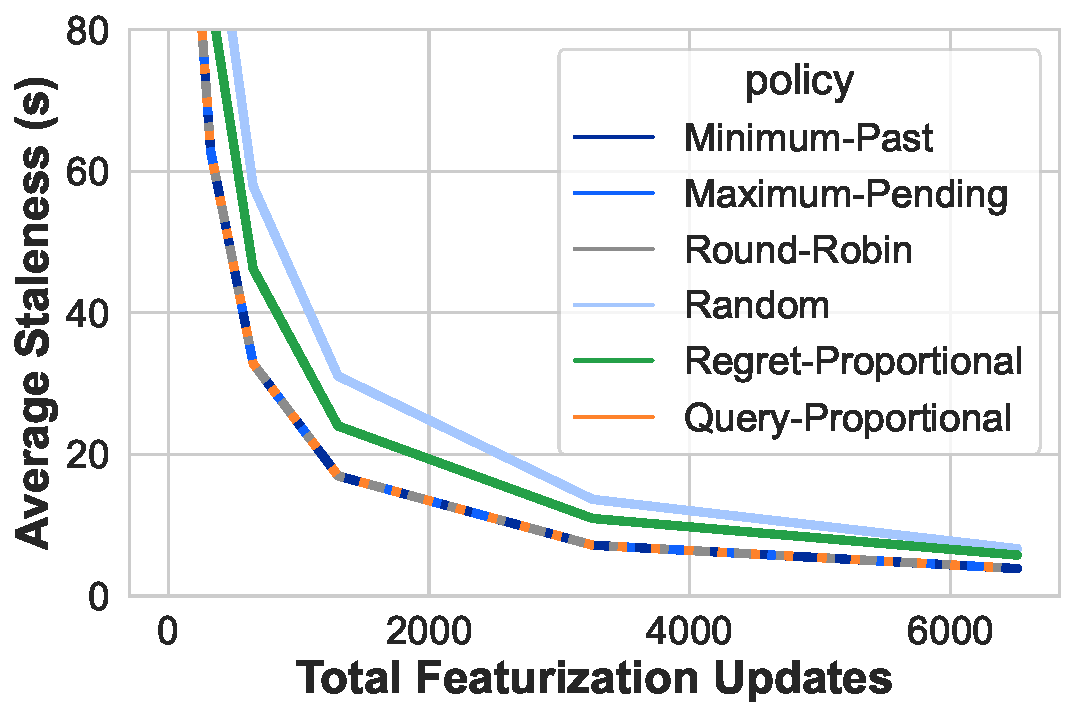
\includegraphics[width=6cm]{ralf/figures/yahoo_a1_results_line_staleness.pdf}
    \caption{\textbf{Queried feature staleness (Anomaly Detection):} Average staleness at query time across key, measured by the number of timesteps since the last update.}
    \label{fig:stl-yahoo-staleness}
\end{figure}

\subsubsection{Query Distributions} 
The Anomaly Detection workload has a uniform query distribution over keys, while for the Recommendation workload, queries for a given user typically come in bursts after long periods of inactivity. We additionally test the effect of different query distributions by re-assinging the inter-arrival times for the Recommendation workloads. We re-assign the inter-arrival times between events to follow an Exponential distribution (equivalent to a poisson process) and a Gaussian distribution, where the mean inter-arrival time is the same as the original distribution. We show in \cref{fig:als-dist} that this leads to similar results as the original distribution of data, showing that Regret-Proportional scheduling is robust to different query distributions. 

\begin{figure}[t]
     \centering
    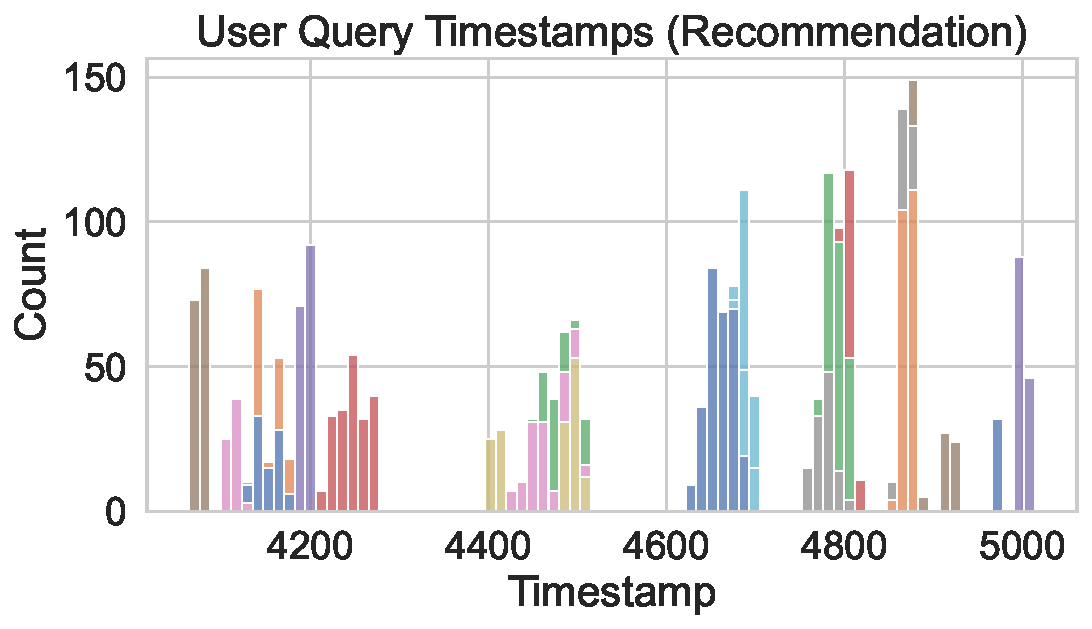
\includegraphics[width=6cm]{ralf/figures/als_user_dist.pdf}
    \caption{\textbf{Frequency of user queries over timestamps.}}
    \label{fig:als-user-dist} 
\end{figure}

\begin{figure}[t]
     \centering
    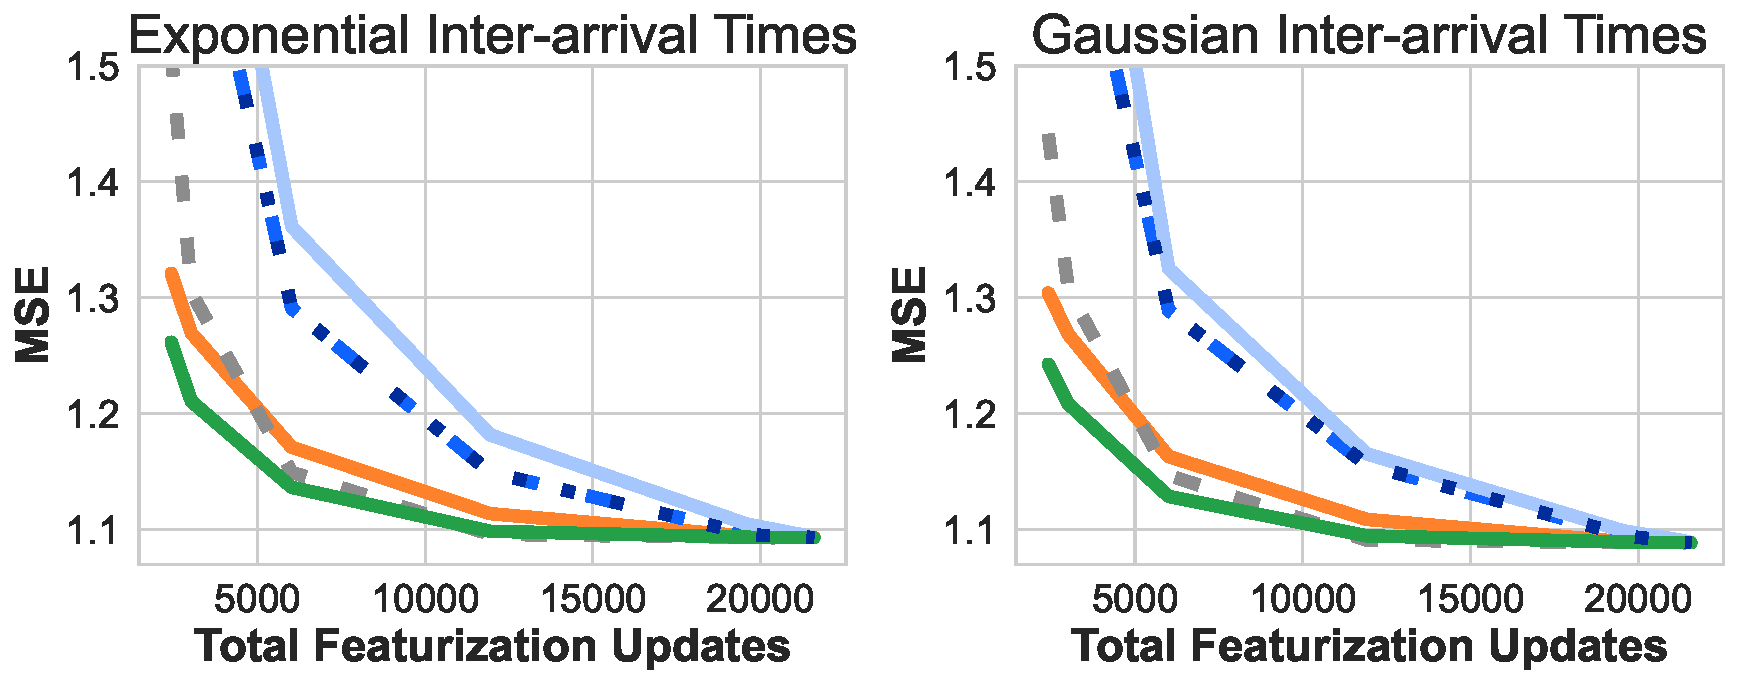
\includegraphics[width=8cm]{ralf/figures/als_dist.pdf}
    \caption{\textbf{Recommendation workload with modified query inter-arrival time shows similar results.}}
    \label{fig:als-dist} 
\end{figure}


\subsection{How well can future error be predicted?}
We evaluate how well error from past queries can predict errors in future queries as a function of the window size of the past queries considered and the lag between the error data and timestamp which we are trying to predict error for (which we refer to as the offset). We train a linear regression model on both the Recommendation and Anomaly Detection workloads to predict error for a future timestep (with some offset) given a window of previous errors for a given key. We show results in \cref{fig:predict_error}, where we plot the MSE of the predicted error. Both workloads benefit from larger windows, but is especially important for the Anomaly Detection workload. Varying the offset hurts the accuracy of the model in Recommendation, suggesting that the freshness of the feedback is critical, while Anomaly Detection relies on just having a sufficient window size (since the per-key error is much more stable over time). 
%These results suggest that the Anonomaly Detection workload could rely on offline regret estimates (described in \cref{ss:online-scheduling-error-feedback}), since the per-key regret is stable, while the Recommendation workload could not. 


\begin{figure}
    \centering
    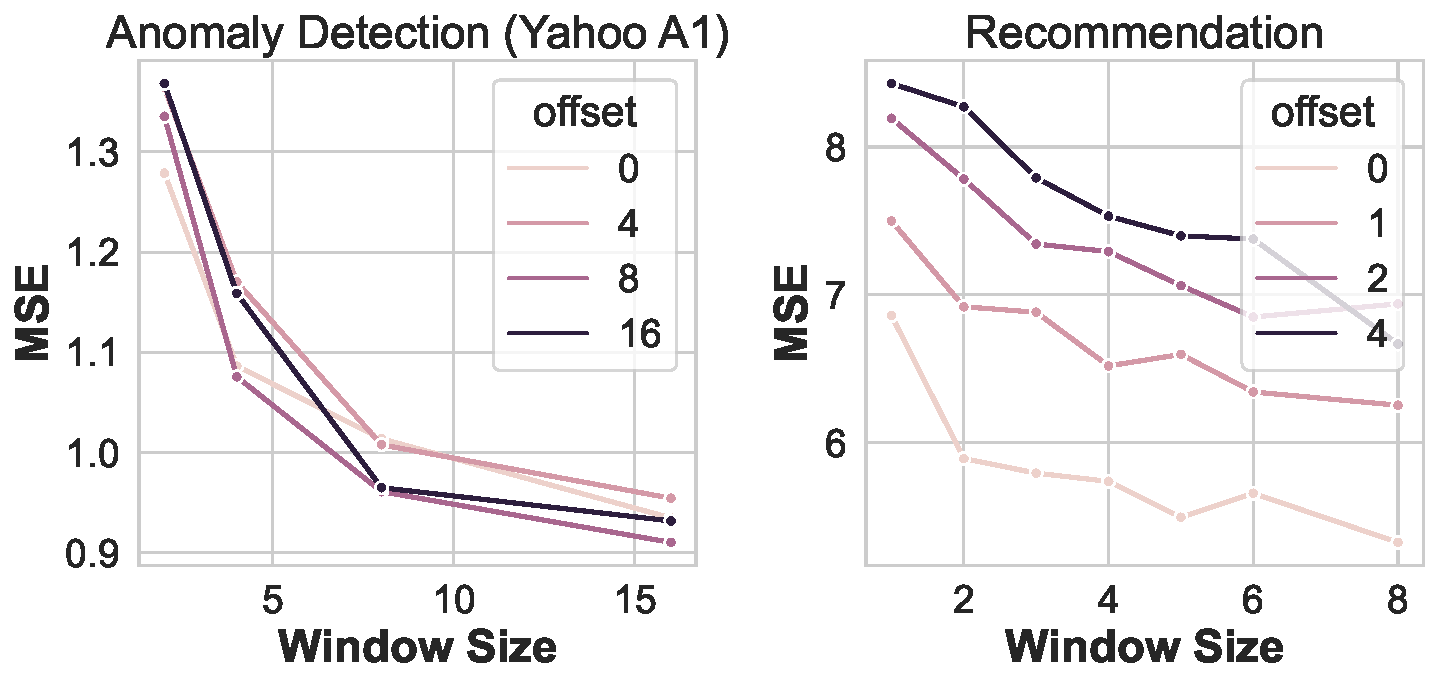
\includegraphics[width=8cm]{ralf/figures/predict_error.pdf}
    \caption{Predicting next timestep error for different window sizes (number of past errors) and offset (timestep delay of the window).}
    \label{fig:predict_error}
\end{figure}


\subsection{Regret-Proportional Scheduling Limitations}
In our workloads, we assume that that the prediction error can be observed and fed back to the scheduler; this allows us to make decisions that will minimize future prediction error by selectively updating certain features. Our purpose in this evaluation is to demonstrate that such feedback from downstream applications---providing recent prediction errors and query patterns--- can be leveraged to make better scheduling decisions for feature maintenance. We believe that future work will be able to make progress is learning to effectively estimate regret from offline data for certain workloads.

There is additionally a concern here with coverage. If we only update features that have incurred past regret, we will fail to update features that have not been queried in the past (e.g. a user who has not logged in in a long time suddenly begins a new session). Such keys form the long tail of the query distribution. To handle this concern, \system{} can be used with a higher default regret value (described in \cref{ss:default-regret}, which will ensure that sufficiently stale keys will eventually be prioritized. However, even without this, since \system{}'s policy is online, so can react quickly to prioritize features that suddenly start to get quried, as shown in our results from the Recommendation workload.




















%%%%%%%%%%%%%%%%%%%%%%%%%%%%%%%%%%%%%%%%%%%%%%%%%%%%%%%%%%%%%%%%%%%%%%%%%%%%
% RELATED WORKS
%%%%%%%%%%%%%%%%%%%%%%%%%%%%%%%%%%%%%%%%%%%%%%%%%%%%%%%%%%%%%%%%%%%%%%%%%%%%
\section{Related Work}
\label{s:related-work}

\myparagraph{Feature Stores} While industry has heavily adopted the use of feature stores~\cite{tecton,hopsworks}, academic research on these systems is limited, and remains focused on metadata and lineage management~\cite{kakantousis2019horizontally}. We discuss feature stores in depth in \cref{s:discussion}.

%While there can been an explosion in the number of feature store projects and companies in industry \cite{tecton}\cite{hopsworks}, there has been limited work on feature stores in academia. Existing work primarily focuses on feature stores in the context of metadata and lineage management \cite{kakantousis2019horizontally}. Recent work by \cite{orr2021managing} proposes the need for managing expensive embeddings, including measuring quality and monitoring model performance. 

\myparagraph{Approximate Query Processing} Approximate query processing reduces the cost and latency of queries by returning approximate results~\cite{agarwal2013blinkdb,chaudhuri2017aqp}. In the machine learning context, recent work investigates how cheaper and more expensive models can be combined to respond to queries \cite{kang2017noscope} while providing formal bounds on approximation~\cite{kang2020approximate}. \system{} focuses on minimizing how frequently feature computation takes place, not on minimizing computation costs. Approximate query processing could be used in conjunction with \system{} to target the latter. Investigating how these two approaches interplay is a promising avenue for future work. 

%\myparagraph{Materialized View Maintenance} Feature tables can be thought of as a materialized view ~\cite{materialized-views} over raw data sources. Prior work in incremental view maintenance and partial view maintenance ~\cite{partially-materialized-views} have examined how to efficiently maintain views over changing data. Noria ~\cite{noria} uses partial state and eventual consistency to efficiently materialize tables both on events and on queries; however, Noria is tightly integrated with SQL and requires commutative, deterministic operators which is too restrictive for many machine learning workloads. In \system{}, we focus on workloads where the primary bottleneck is a 1-to-many \sarah{is there a better word for "1-to-many" map function over keys?} map function, where the output table is directly queried by the downstream application. Adding multiple materialized views, joins, and incremental updates would be interesting variation to add to \system{}'s policies in future work. 
%\natacha{Mention Timely and Materialize? They are the ones that really focus on incremental view maintenance and on efficient recomputation}

\myparagraph{Materialized View Maintenance}
 Feature tables can be thought of as a materialized view ~\cite{materialized-views} over raw data sources. Prior work in incremental view maintenance and partial view maintenance ~\cite{partially-materialized-views} have examined how to efficiently maintain views over changing data. Noria ~\cite{noria} uses partial state and eventual consistency to efficiently materialize tables both on events and on queries. Timely Dataflow~\cite{timely-dataflow-book} leverages shared arrangements~\cite{DBLP:journals/pvldb/McSherryLSR20} to facilitate incremental recomputation of a view. No existing work focuses on \textit{when} to recompute a given view and how to prioritize across view to optimize application correctness. 

\myparagraph{Prediction Serving} Most prior work in prediction serving \cite{clipper,crankshaw2020inferline} focuses on optimizing model
serving resource efficiency but does not consider the feature stores in
such pipelines; these systems exclusively target improving model inference and fail to consider data preprocessing and featurization. Systems
that do consider featurization either focus on making use of cheaper 
featurization functions which can be approximated without affecting prediction~\cite{willump}, or target specific application use cases such as video analytics~\cite{li2020towards,jiang2018chameleon,bhardwaj2020ekya}.

%However prior work does not consider prediction serving pipelines with feature stores, primarily focuses on optimizing model inference rather than data preprocessing and featurization. 
%Some work in serving has focused on join optimization of featurizaiton and inference \cite{kang2020jointly} \cite{kraft2019willump}. Willup uses cheaper featurization functions for features which can be approximated without significantly affecting the prediction result (e.g. for "easy" inputs, of top-K queries) to reduce model inference cost. However Willump does not explore the tradeoffs with using stale features, and focuses on approximating the computation. Prior work in inference over video streams has considered the effect of stale object prediction on downstream tasks \cite{li2020towards}, but is specific to the context of streaming inference on video. Work in video analytics has also explored real-time adaptation of video analytics pipelines with periodic profiling \cite{jiang2018chameleon}\cite{bhardwaj2020ekya}, but is also specific to video analytics and cannot be applied to evaluating and configuring feature stores. 

%\myparagraph{Feature Selection} Prior work such as Pyramid ~\cite{lecuyer2017pyramid} has examined how subsets of data can be selected to reduce privacy risk of data being trained on. \natacha{I would remove, not necessary I don't think}

%\myparagraph{OLTP/OLAP} \natacha{I would remove, not necessary I don't think}

\myparagraph{Staleness and Consistency} Trading-off consistency for performance is a well-known strategy in modern large-scale distributed systems. These key-value stores or databases relax constraints on when and how operations must take effect, reducing the cost of synchronization~\cite{cooper2008pnuts,lloyd2011cops,sivasubramanian2012amazon, lloyd2011cops,bailis2012pbs,terry2013pileus,yu2022conit,cui2014bounded}. The flip-side is the increased programmer burden in defending against the potential unexpected application behaviours that arise from these relaxed guarantees~\cite{crooks2016tardis, bailis2012pbs}. To minimize this issue, prior work either 1) distinguishes between operations whose ordering can be safely relaxed~\cite{li2012redblue, kraska2013mdcc, bailis20iva} 2) bounds divergence from the true value when possible~\cite{yu2022conit,holt2016disciplined, wu1992divergence, cui2014bounded, wong1992bounded}. The former is often restrictive, while the latter does not discuss the application-level consequences of diverging from the true value. These limitations have led to skepticism as to whether weak consistency is valuable option for developers. Feature store systems, in contrast, have \textit{explicit} metrics and mechanisms to understand loss of correctness; they are thus uniquely positioned to leverage weak consistency and the staless/consistency tradeoff that it enables. 

%\myparagraph{Streaming dataflow systems} \natacha{Would remove, not saying something especially interesting right now, and you could have easily implemented your system on top of them. You say in Sec 2 that you could, I suspect that's enough? I would disagree with Joe, to me the implementation is pretty important rather than the API as they make very different tradeoffs (timely vs Noria is pretty fundamental for ex), but not necessary or now? }
%\jmh{Again, I think this is a big old red herring. You can almost certainly use any dataflow system to express the mappings you want from inputs to outputs; the good stuff you're doing it the (re-)parameterization of those mappings over time. I feel like you are calling out to these systems to appease somebody, when at the end of the day what matters is the choice of dataflow/query you write in these systems, not the implementation of the systems. Personally I think relational languages (algebra, SQL, etc) are a fine choice since you want to express at each update an arbitrary mapping from input data to output features; various ``query templates'' capture the properties of the mapping--the relation!--between inputs and outputs over time in a way you could characterize nicely. ANyhow, I recommend that you stay above the fray and argue for the intrinsic value (and portability!) of setting up and solving the proper optimization problem.}
%


%\myparagraph{Model Training}
% Chameleon
% - dynamically picks best configuration for ML video analytics pipelines.
% - computes accuracy relative to a "golden configuration".
% - reconfigures pipelines using similarities to trim the search space,
%   rather than prioritizing computation.
% Ekya
% - Uses profiler to select models on edge video analytics systems to retrain.
% - Mitigates data drift, navigates tradeoff b/t retrained model accuracy and inference accuracy.
% Clipper
% - Uses adaptive online model selection to improve accuracy.
% - Attempts to meet throughput and latency SLOs
% - Does not prioritize/deprioritize per-key features to reduce resource
%   consumption while maintaining high accuracy.
% Inferline
% - Manages stages of a prediction pipeline to meet e2e tail latency constraints and minimize cost.
% - Inferline tuner responds to changes in query patterns.
% - Doesn't focus on e2e accuracy of the application.
% SEDA
% - Consists of stages, similar to RALF operators.
% - Provides control mechanisms for automatic tuning and load conditioning of each stage,
%   similar to RALF per-operator prioritization policies.
% - Not aware of e2e accuracy, focuses on xput, response time, fairness to clients.
% Willump
% - Uses cascades to classify and quickly generate features for "easy" data, falling back to more expensive models.
% - Optimizes top-k queries using approximation to filter out low-scoring inputs.
% Parameter server
% TODO?

% Systems for continual learning have explored cost accuracy tradeoffs with model training for specific applications. Recent work explores optimizing accuracy for video analytics on edge 
% devices~\cite{chameleon,ekya}, by balancing resource allocation between training and serving. However, the solutions rely on close observations of
% specific application characteristics. 
%



%%%%%%%%%%%%%%%%%%%%%%%%%%%%%%%%%%%%%%%%%%%%%%%%%%%%%%%%%%%%%%%%%%%%%%%%%%%%
% Discussion
%%%%%%%%%%%%%%%%%%%%%%%%%%%%%%%%%%%%%%%%%%%%%%%%%%%%%%%%%%%%%%%%%%%%%%%%%%%%
\section{Discussion}
\label{s:discussion}
In this paper we focused on feature stores in the context of online serving and real-time maintenance for staleness-sensitive features. However, real-world deployments of feature stores have diverse requirements, design choices, and applications in ML pipelines. 

\subsection{Feature Materialization}

Most feature stores do not support feature materialization, and instead support ingestion of pre-computed features through streaming and batch ingest pipelines. Other feature stores (e.g. Tecton) offer built-in transformation tools. Existing feature transformation systems are usually built on top of multiple existing computational engines (e.g. Flink, Spark, AWS lambda) to support different ways of materializing features, making it difficult to apply general optimization techniques across them.

For feature stores that support materialization (e.g. Tecton), there are typically three types of feature materialization: 
\begin{enumerate}
    \item \textbf{Batch}: Features are periodically refreshed (e.g. daily, hourly) with a batch processing system (e.g. Spark, Airflow). 
    \item \textbf{Streaming}: Features are continually re-computed with new data arriving in a streaming fashion with a streaming system (e.g. Flink, Spark Streaming). 
    \item \textbf{On-Demand (i.e. Lazy)}: The feature is materialized at query time (e.g. with a lambda function).
\end{enumerate}
Whether feature should be pre-materialized or materialized in real-time depends on the cost of featurization, the query latency requirements, and the rate of incoming new data and queries. Batch feature updates can be more cost effective for features which are not staleness sensitive. On-demand feature updates are cost effective when the latency of the feature computation is very low or there is not a requirement for low-latency queries. 

Although we primarily focused on the case of steaming materialization of expensive features, the policies in \system{} can be applied to any case where only a subset of keys can be processed. This applies to both streaming materialization and batch materialization where the throughput may be limited. 

Prior work in approximate query processing and approximate featurization \cite{willump} can also reduce the cost of feature materialization and be used in conjunction with batch, streaming, or on-demand materialization. We consider this line of work orthogonal, as both key-prioritization and feature approximation can be combined to reduce cost.  
\sarah{this is a new section, please review}
\joey{I like it!}


\sarah{TODO: explicitly outline the types of featurization (batch, streaming, on-demand) and how they relate to FLAR. Remove sentence about "batch processing" being out of scope).}
\joey{This is resolved now right?}

%A challenge for streaming materialization of feature is the high-cardinality of many feature tables \textcolor{red}{(TODO: cite splunk paper} An e-commerce website could be storing feature for millions of users. As a result, even if the true feature values for each key as changing slowly, continually updating every feature value with new data can be computationally infeasible. Furthermore, data for all keys may not fit into memory, necessitating that only a subset of keys are updated at once. 

\subsection{Feature Storage}
Feature stores are typically responsible for serving features to online model serving pipelines with low latency, as well as storing large amounts of historical data and features for model training pipelines. As a result, feature stores typically contain two separate datastores: 1. an \textit{offline store} for offline training, and 2. a \textit{online store} online model serving. The offline store is usually a high-throughput, high-latency storage systems like cloud object stores or data lakes. The online store, however, must serve features with tight latency constraints (on the order of 100s of milliseconds). As a result, a smaller subset of features are often stored in in-memory K/V stores (e.g. Redis \cite{redis}).

One challenge with splitting feature storage between separate online and offline stores is maintaining \textit{offline/online consistency}. Differences in the ways that features are ingested, materialized, or defined between the offline and online store results in slightly different sets of features being served to training pipelines and inference pipelines. Slight differences in features can results in \textit{data drift} for models, which can cause significant depredations in prediction accuracy. As a result, some feature stores will only allow direct updates to either the offline or online store, and syncs values from one store to another. While this approach can reduce the risk of data drift, synchronization can incur additional overhead and latency in updating features. In this paper, we only focused on materialization for the online store (as we focused on prediction serving), however future work should explore how scheduling policies could affect online and offline consistency. 


\subsection{Limitations of Existing Feature Stores}
Despite being designed for machine learning workloads, existing feature store systems do not account for accuracy in how they maintain feature values. Feature store are uniquely situated between updates to features and feature queried, but typically lack awareness of downstream query patterns and performance of the predictions made using queried features. As a result, systems for maintaining features treat all data updates and keys symmetrically and fail to leverage important information about which updates are critical and which keys are likely to be accessed in the downstream prediction workload. In the online setting, these systems make only a best-effort attempt at maintaining feature values up-to date. Features might become arbitrary stale, significantly hurting accuracy. While the cost of computing features in the online setting excludes keeping features, fully up-to-date, we find the current approach suboptimal. 

%In this paper, we design a prototype feature store to estimate downstream accuracy impact of keys to intelligently schedule feature updates. We demonstrate that accuracy-aware scheduling of updates can satisfy our stated objective: build a resource efficient feature store. 







%%%%%%%%%%%%%%%%%%%%%%%%%%%%%%%%%%%%%%%%%%%%%%%%%%%%%%%%%%%%%%%%%%%%%%%%%%%%
% CONCLUSIONS
%%%%%%%%%%%%%%%%%%%%%%%%%%%%%%%%%%%%%%%%%%%%%%%%%%%%%%%%%%%%%%%%%%%%%%%%%%%%
\section{Conclusion}
\label{s:conclusions}

In this paper, we studied the challenge of feature maintenance in feature stores, an emerging new class of systems.
First, we identified a critical limitation in existing approaches to feature store design: current feature stores treat data and keys symmetrically and do not leverage crucial signal about query access patterns or the impact of features on downstream task performance.
We then formalized the feature store problem and introduced \textit{feature store regret}, a metric that measures the impact of staleness of features on the downstream prediction accuracy.
Finally, we presented \system{}, a feature store system that uses prediction loss as feedback to prioritize updates that improve the downstream accuracy via Regret-Proportional scheduling.
Experiments on a range of feature maintenance policies demonstrate that prioritizing replacing features with the highest \textit{cumulative regret} can significantly improve prediction accuracy in resource-constrained settings. We believe this paper will provide a formal foundation for a key problem in the emerging class of feature store systems and hope that it will inspire future work in the design of more advanced feature maintenance strategies.
% \begin{itemize}
%     \item Co-scheduling queries and updates 
%     \item Sharing state 
% \end{itemize}


%\begin{acks}
%This work was supported by gifts from AMD, Anyscale, Astronomer, Google, IBM, Intel, Lacework, Microsoft, Samsung SDS, Uber, and VMware. We also thank Abhinav Mishra and Ram Sriharsha for help with understanding feature store challenges at Splunk. 
%\end{acks}



%\begin{table*}[t]
%  \caption{A double column table.}
%  \label{tab:commands}
%  \begin{tabular}{ccl}
%    \toprule
%    A Wide Command Column & A Random Number & Comments\\
%    \midrule
%    \verb|\tabular| & 100& The content of a table \\
%    \verb|\table|  & 300 & For floating tables within a single column\\
%    \verb|\table*| & 400 & For wider floating tables that span two columns\\
%    \bottomrule
%  \end{tabular}
%\end{table*}

% \begin{acks}
%  This work was supported by the [...] Research Fund of [...] (Number [...]). Additional funding was provided by [...] and [...]. We also thank [...] for contributing [...].
% \end{acks}

%\clearpage

%\bibliographystyle{ACM-Reference-Format}
%\bibliography{sample}

%\end{document}
%\endinput

% cloudcast 

\bibliography{thesis}{}

\end{document}
